% =====================================================================
%  LineSense AI -- project report
%
%  Build:  scripts/heavy-job.sh tectonic docs/report/linesense-report.tex
%  Engine: Tectonic 0.17.0 (XeTeX). Any pdfLaTeX/XeLaTeX run also works.
%
%  Template gap: the official IT 3041 report template was never supplied to
%  this project. This document is self-structured; restructure it into the
%  official template when it becomes available. See section 1.2.
% =====================================================================
\documentclass[11pt,a4paper]{article}

\usepackage[T1]{fontenc}
\usepackage{lmodern}
\usepackage{amsmath}
\usepackage{amssymb}
\usepackage[a4paper,top=2.3cm,bottom=2.3cm,left=2.2cm,right=2.2cm]{geometry}
\usepackage{microtype}
\usepackage{graphicx}
\usepackage{tikz}
\usepackage{pdflscape}
\usepackage{booktabs}
\usepackage{longtable}
\usepackage{array}
\usepackage{tabularx}
\usepackage{xcolor}
\usepackage{enumitem}
\usepackage{caption}
\usepackage{fancyhdr}
\usepackage{parskip}
\usepackage[hidelinks]{hyperref}

% Shared TikZ styles for every LineSense report diagram.
% Input once from the preamble of docs/report/linesense-report.tex.
%
% Layout rules every diagram in this directory follows:
%   * nodes are placed on an explicit coordinate grid (or with `positioning`
%     at fixed distances), never by an automatic layout engine;
%   * every connector is orthogonal -- pure vertical/horizontal segments, or
%     TikZ's `-|` / `|-` routing;
%   * every edge label is a node with `midway`/`pos=`, drawn with an opaque
%     white background so a label never sits on top of a line;
%   * node widths are fixed, so boxes in the same row can never overlap.

\usetikzlibrary{arrows.meta,positioning,fit,backgrounds,shapes.geometric,%
                shapes.multipart,calc,decorations.pathreplacing,patterns}

\definecolor{lsblue}{HTML}{1F4E79}
\definecolor{lsblued}{HTML}{DCE6F2}
\definecolor{lsgreen}{HTML}{2E6F40}
\definecolor{lsgreend}{HTML}{DCEEDF}
\definecolor{lsamber}{HTML}{8A5A00}
\definecolor{lsamberd}{HTML}{FBEBCF}
\definecolor{lsgrey}{HTML}{4D4D4D}
\definecolor{lsgreyd}{HTML}{ECECEC}
\definecolor{lsred}{HTML}{8B2020}
\definecolor{lsredd}{HTML}{F7DDDD}

% Hyphenation inside a narrow node box produces ugly "ap-\\plies" breaks and
% can push a word over a neighbouring node, so it is switched off for every
% node style below (body text keeps normal hyphenation).
\newcommand{\nohyph}{\hyphenpenalty=10000\exhyphenpenalty=10000\relax}

\tikzset{
  lsbox/.style        = {draw, rounded corners=2pt, align=center,
                         font=\scriptsize\nohyph, inner sep=3pt,
                         minimum height=1.25cm, text width=3.0cm},
  person/.style       = {lsbox, draw=lsblue, fill=lsblued, line width=0.5pt},
  system/.style       = {lsbox, draw=lsblue, fill=lsblue!25, line width=0.9pt,
                         font=\scriptsize\bfseries\nohyph},
  container/.style    = {lsbox, draw=lsblue, fill=lsblued, line width=0.7pt},
  component/.style    = {lsbox, draw=lsgreen, fill=lsgreend, line width=0.5pt},
  store/.style        = {lsbox, draw=lsamber, fill=lsamberd, line width=0.7pt},
  external/.style     = {lsbox, draw=lsgrey, fill=lsgreyd, line width=0.5pt},
  danger/.style       = {lsbox, draw=lsred,  fill=lsredd,  line width=0.6pt},
  %
  state/.style        = {draw=lsblue, fill=lsblued, rounded corners=7pt,
                         align=center, font=\scriptsize\nohyph, inner sep=3pt,
                         minimum height=0.85cm, text width=2.5cm},
  terminal/.style     = {state, draw=lsgreen, fill=lsgreend},
  badstate/.style     = {state, draw=lsred,  fill=lsredd},
  choice/.style       = {draw=lsamber, fill=lsamberd, diamond, aspect=2.1,
                         align=center, font=\tiny\nohyph, inner sep=1.5pt},
  dot/.style          = {circle, fill=lsblue, minimum size=3.2mm, inner sep=0pt},
  %
  flow/.style         = {-{Stealth[length=2.0mm,width=1.6mm]}, draw=lsgrey,
                         line width=0.55pt},
  biflow/.style       = {{Stealth[length=2.0mm,width=1.6mm]}-%
                         {Stealth[length=2.0mm,width=1.6mm]},
                         draw=lsgrey, line width=0.55pt},
  reply/.style        = {flow, dashed, dash pattern=on 2pt off 1.4pt},
  trans/.style        = {-{Stealth[length=2.0mm,width=1.6mm]}, draw=lsblue,
                         line width=0.6pt},
  badtrans/.style     = {-{Stealth[length=2.0mm,width=1.6mm]}, draw=lsred,
                         line width=0.6pt},
  lifeline/.style     = {draw=lsgrey!60, dashed, dash pattern=on 1.6pt off 1.6pt,
                         line width=0.4pt},
  %
  lbl/.style          = {font=\tiny\nohyph, fill=white, inner sep=1.4pt,
                         align=center, text=black},
  lblw/.style         = {lbl, text width=2.6cm},
  lblx/.style         = {lbl, text width=3.4cm},
  note/.style         = {font=\tiny\itshape\nohyph, align=left, text=lsgrey,
                         fill=white, inner sep=2pt},
  boundary/.style     = {draw=lsblue!55, dashed, rounded corners=5pt,
                         line width=0.6pt, inner sep=9pt},
  boundlbl/.style     = {font=\tiny\bfseries\nohyph, text=lsblue, inner sep=2pt,
                         align=left},
}


\newcolumntype{L}[1]{>{\raggedright\arraybackslash}p{#1}}
\newcolumntype{Y}{>{\raggedright\arraybackslash}X}

% Long \texttt{} identifiers are the main source of overfull lines in narrow
% table cells; allow generous inter-word stretch rather than shrinking the font.
\emergencystretch=3.5em
\sloppy
\hbadness=6000

\captionsetup{font=small,labelfont=bf}
\setlist[itemize]{topsep=2pt,itemsep=1pt,parsep=0pt,leftmargin=1.3em}
\setlist[enumerate]{topsep=2pt,itemsep=1pt,parsep=0pt,leftmargin=1.6em}

\pagestyle{fancy}
\fancyhf{}
\fancyhead[L]{\small LineSense AI -- project report}
\fancyhead[R]{\small\thepage}
\renewcommand{\headrulewidth}{0.3pt}

% Honest-status callout box.
\newcommand{\statusbox}[2]{%
  \begin{center}
  \fcolorbox{lsred}{lsredd}{%
    \begin{minipage}{0.95\linewidth}\small\textbf{#1}\\[2pt]#2\end{minipage}}
  \end{center}}
\newcommand{\notebox}[2]{%
  \begin{center}
  \fcolorbox{lsblue}{lsblued}{%
    \begin{minipage}{0.95\linewidth}\small\textbf{#1}\\[2pt]#2\end{minipage}}
  \end{center}}

% Convenience macros for the two page-wide landscape diagrams.
\newcommand{\widefig}[3]{%
  \begin{landscape}
  \begin{figure}[p]
  \centering
  \resizebox{!}{#3\textheight}{\input{diagrams/#1}}
  \caption{#2}
  \end{figure}
  \end{landscape}}

\hypersetup{pdftitle={LineSense AI -- project report},
            pdfsubject={IT 3041 group assignment}}

\begin{document}
\thispagestyle{empty}

\begin{center}
  {\Huge\bfseries LineSense AI}\\[10pt]
  {\large A factory operations decision-support system for apparel
   manufacturing:\\[3pt] four bounded agents over a deterministic domain core}\\[20pt]
  {\normalsize IT 3041 group assignment}\\[6pt]
  {\small\itshape Author names and student numbers to be completed by the team
   before submission\\ (see \texttt{docs/assessment/contribution-log.md})}\\[10pt]
  {\small 20 September 2026}
\end{center}
\vspace{6pt}

\statusbox{Read this before any number in this report}{%
This report describes a system that was really built and really tested, but
\emph{not} everything in it has been executed. Three things in particular have
never run in the environment that produced this repository, and are marked as
such wherever they appear:
\begin{itemize}
\item \textbf{No live language-model call has ever been made.} No provider API
  key exists here. Every agent run in this project used the deterministic
  \texttt{fixture} provider, labelled \emph{``Test fixture --- not a live AI
  model''} in the UI, in the API and in every evaluation artefact.
\item \textbf{No Docker image was ever built or started.} The Compose, Caddy
  and Keycloak artefacts were validated \emph{statically} only.
\item \textbf{The full evaluation, the load test, and the full test suites were
  not run locally}, under this project's machine heat and workload policy. Each
  is listed as \textbf{PENDING (needs user approval or CI)} with the exact
  command that would produce it.
\end{itemize}
Browser end-to-end testing was \textbf{dropped by the user} as a scope
decision, so there is no Playwright suite, no \texttt{make test-e2e} target and
\textbf{no screenshots} anywhere in this submission.}

\vfill
\noindent\small
Repository: \texttt{feat/linesense-build}. The running, dated log of what was
built and what was actually run is \texttt{docs/IMPLEMENTATION\_STATUS.md}; the
requirement-by-requirement verdict is
\texttt{docs/assessment/completion-matrix.md}.

\clearpage
\tableofcontents
\clearpage

% =====================================================================
\section{Introduction and problem}
% =====================================================================

\subsection{The problem}

An apparel factory answers the same question dozens of times a day, and answers
it badly: \emph{can this order finish on time, what is blocking it, what
evidence supports that, and what should we do next?} The information needed to
answer it is real and already exists --- order books, bills of material, stock
ledgers, line capacity calendars, cycle-time observations, inspection records,
standard operating procedures --- but it sits in different spreadsheets, a
partially-used ERP, a storekeeper's notebook and an industrial engineer's
clipboard. Reconciling it is manual, slow, and done under time pressure by the
person least able to spare the time.

The consequence is not usually a wrong decision. It is a \emph{late} decision:
a material shortage discovered on the day the line was supposed to start, a
bottleneck operation nobody quantified, a quality hold that was not visible to
the person promising a shipping date.

\subsection{What LineSense AI is}

LineSense AI is a decision-support application for that question. Four bounded
AI agents --- \textbf{planning/allocation}, \textbf{raw materials (RM)},
\textbf{industrial engineering (IE)/cycle time} and \textbf{quality} ---
investigate one order, each using scoped read-only tools over a deterministic
domain core, and produce evidence-linked findings. Anything they propose is a
\emph{recommendation}, never a change: a second human being must approve it and
then apply it through a transaction that re-checks every input version before it
writes anything.

Three design commitments run through the whole system and are the reason it can
be trusted at all:

\begin{enumerate}
\item \textbf{A language model never establishes business truth.} Stock,
  capacity, cycle times, quality eligibility and lifecycle transitions are
  computed by pure Python in \texttt{app/domain/} --- \texttt{Decimal} in,
  \texttt{Decimal} out, no I/O. A model may explain a result, pick one of the
  options the deterministic code already produced, and cite evidence that
  already exists. It cannot produce a number, a state, or a verdict.
\item \textbf{Every consequential action is a proposal until a human approves
  it.} The proposer may not approve their own proposal; an approval does not
  apply anything; and an application that finds any input has moved fails
  closed.
\item \textbf{Nothing is shown without its source.} Every value on screen is
  labelled \emph{``Calculated from records''}, \emph{``AI recommendation''},
  \emph{``Test fixture --- not a live AI model''}, \emph{``AI disabled ---
  deterministic results only''}, \emph{``Pending human approval''} or
  \emph{``Approved by [role/user] at [time]''}.
\end{enumerate}

The system recommends. It does not operate machinery, place purchase orders, or
authorise shipments.

\subsection{Template gap and the honesty rule this report follows}
\label{sec:template-gap}

\textbf{The official report template was not supplied to this project.} This
document is self-structured; when the template becomes available, restructure
this content into it rather than rewriting the content.

Every quantitative claim below cites the artefact that produced it --- a
recorded command in \texttt{docs/IMPLEMENTATION\_STATUS.md}, a test name, a
generated document, or a file in the repository. Anything that was not executed
is named as not executed. Section~\ref{sec:not-verified} is a single list of
everything in this category, and the completion matrix
(\texttt{docs/assessment/completion-matrix.md}) repeats the verdict per
requirement.

% =====================================================================
\section{Domain, users and roles}
% =====================================================================

\subsection{Demonstration domain}

The demonstration organization is \emph{Demo Apparel Group} with two factories,
\texttt{KTN} (Katunayake Plant) and \texttt{BYG} (Biyagama Plant). Two factories
exist specifically so that access boundaries can be tested: a planner at BYG
must not be able to see a KTN order, and a negative test asserts they receive
\texttt{404}, not \texttt{403} --- the existence of an out-of-scope resource is
never revealed.

All data is synthetic and generated deterministically
(\texttt{app/seed/generator.py}, seed \texttt{20260917}). Every customer name is
obviously fictional (\emph{Customer 07 Apparel Co.}); every worker identifier is
a pseudonymous alias code (\texttt{KTN-OP-014}), never a person's name.

\begin{table}[h]
\centering\small
\caption{The seeded demonstration dataset (\texttt{docs/evaluation/synthetic-data.md}).}
\begin{tabular}{@{}lr@{\hspace{2.2em}}lr@{}}
\toprule
Organizations / factories & 1 / 2 & Capacity slots (9 lines $\times$ 30 d $\times$ 2 shifts) & 540\\
Users / memberships / role assignments & 10 & Orders (80 KTN, 20 BYG, 1 demo) & 101\\
Customers & 26 & Allocations & $\approx$160\\
Styles / style operations & 12 / $\approx$88 & Material lots / movements / balances & 40 / $\approx$600 / 40\\
Materials & 20 & Reservations / expected receipts & $\approx$75 / $\approx$11\\
BOM versions / lines & 16 / $\approx$61 & Operator aliases / skill records & 150 / $\approx$300\\
Production lines (KTN L1--L6, BYG B1--B3) & 9 & Cycle observations / line measurements & 720 / $\approx$108\\
SOP corpus documents & 30 & Inspections / defects / holds / releases & $\approx$40 / $\approx$32 / 1 / $\approx$18\\
\bottomrule
\end{tabular}
\end{table}

\subsection{Roles}

Roles are \textbf{additive and explicit}. Nothing is implied: an
\texttt{org\_admin} administers membership and configuration and has \emph{no}
business authority --- it cannot approve a recommendation, transition an order,
or write inventory, IE or quality records. The authoritative matrix is generated
from the code (\texttt{scripts/gen\_role\_matrix.py} reads
\texttt{app.auth.policy.PERMISSIONS}) and is reproduced in
Appendix~\ref{app:roles}.

\begin{table}[h]
\centering\small
\caption{The seven roles and what each may do beyond the shared read set.}
\begin{tabularx}{\linewidth}{@{}lY@{}}
\toprule
\textbf{Role} & \textbf{Authority beyond reading}\\
\midrule
\texttt{viewer} & none --- authorized read-only dashboards and evidence\\
\texttt{planner} & create/import orders, transition orders, \emph{start an analysis run}, add notes\\
\texttt{storekeeper} & material receipts, lot acceptance, issues, corrections, reservations and releases\\
\texttt{ie\_engineer} & record cycle observations, mark an outlier, upload documents\\
\texttt{quality\_manager} & record inspections, place holds, record releases, upload documents\\
\texttt{supervisor} & everything a planner may do, plus \emph{decide} and \emph{apply} recommendations, cancel/dispatch orders, read the audit log, upload documents\\
\texttt{org\_admin} & membership and role administration, audit log, policy list, effective run limits --- and no business authority at all\\
\bottomrule
\end{tabularx}
\end{table}

Two supervisors and two quality managers are seeded deliberately: separation of
duties requires a second person. The proposer of an analysis can never approve
or apply the resulting recommendation, and a quality manager can never release
an order against an inspection they recorded themselves.

% =====================================================================
\section{Requirements}
% =====================================================================

\texttt{docs/requirements.md} is the requirements baseline: 21 numbered
functional requirements (\texttt{REQ-01}\dots\texttt{REQ-21}) and 5
non-functional requirements (\texttt{NFR-01}\dots\texttt{NFR-05}), each with
acceptance criteria and a ``where implemented'' pointer. Every one of them is
carried into \texttt{docs/assessment/completion-matrix.md} with a verdict of
\emph{Met}, \emph{Partially met}, \emph{Not verified} or \emph{Not met} and a
link to the evidence.

\begin{table}[h]
\centering\small
\caption{Assignment requirement $\rightarrow$ implementation $\rightarrow$ evidence.}
\begin{tabularx}{\linewidth}{@{}L{3.1cm}YL{3.6cm}@{}}
\toprule
\textbf{Brief requirement} & \textbf{What was built} & \textbf{Evidence}\\
\midrule
Two or more interacting intelligent agents &
Four domain agents exchanging typed tasks and results through an orchestrated,
versioned HTTP/JSON protocol; planning consumes RM and IE results and is
re-dispatched when RM contradicts it &
\texttt{tests/integration/test\_four\_agent\_flow.py}, \texttt{test\_two\_agent\_flow.py}; figure~\ref{fig:seq}\\
LLM use &
One \texttt{LLMClient} boundary; the model selects among offered tools, writes
the explanation and picks one of the deterministic candidate actions &
\texttt{app/llm/}, \texttt{docs/architecture/llm-boundary.md}. \textbf{Live provider never exercised}\\
NLP &
Entity extraction over authorized master data, note classification, grounded
summaries &
\texttt{app/nlp/}; micro-F1 0.991 / macro-F1 0.835 on the held-out split (smoke run, \S\ref{sec:eval})\\
Information retrieval &
Lexical \texttt{tsvector} + pgvector cosine, fused by reciprocal-rank fusion,
filtered by organization/factory/ACL/version before content reaches a model &
\texttt{app/retrieval/}; figure~\ref{fig:docs}; \S\ref{sec:eval}\\
Security &
OIDC + PKCE, opaque server sessions, CSRF double-check, scoped authorization on
every path, validated uploads, rate limits, audit &
\texttt{tests/security/} (7 modules), \texttt{docs/security/threat-model.md}\\
Defined agent protocol &
\texttt{schema\_version "1.0"} envelope/result over
\texttt{POST /internal/v1/agent-tasks} with a service token &
\texttt{contracts/agent-task-envelope.schema.json}, \texttt{contracts/agent-result.schema.json}\\
Responsible AI &
Evidence-linked findings, abstention, pseudonymous worker data, human review of
every consequential action &
\texttt{docs/assessment/responsible-ai.md}, \texttt{model-card.md}, \texttt{data-card.md}\\
Commercialization &
Target market, three tiers, cost model, deployment options, pilot plan &
\texttt{docs/assessment/commercialization.md}, \S\ref{sec:commercial}\\
\bottomrule
\end{tabularx}
\end{table}

% =====================================================================
\section{System design}
% =====================================================================

\subsection{Architectural style}

LineSense is a \textbf{modular monolith with a separate worker process}
(ADR-0001). The four agents are independently specified software components
inside one backend codebase; none of them is a deployed microservice. The
reasons are recorded in the ADR: at this scale, per-agent services would add
deployment, failure and consistency modes without adding capability, and the
protocol boundary that matters --- a versioned message contract with tenant
scoping, budgets and evidence rules --- can be enforced just as strictly inside
one process boundary.

One PostgreSQL 16 cluster with the \texttt{pgvector} extension is the only
datastore (ADR-0002): domain data, the job queue, run records, the audit log and
the chunk embeddings all live in it. There is no separate vector database, no
Kafka, no Redis and no Kubernetes.

\begin{figure}[p]
\centering
\resizebox{\textwidth}{!}{% C4 level 1 -- system context.
% Grid: people on row y=4.6, the system at y=0, external systems at y=-4.6.
% Every connector is a pure vertical segment (x of the actor == x of its
% entry point on the system box), so no arrow can cross a node.
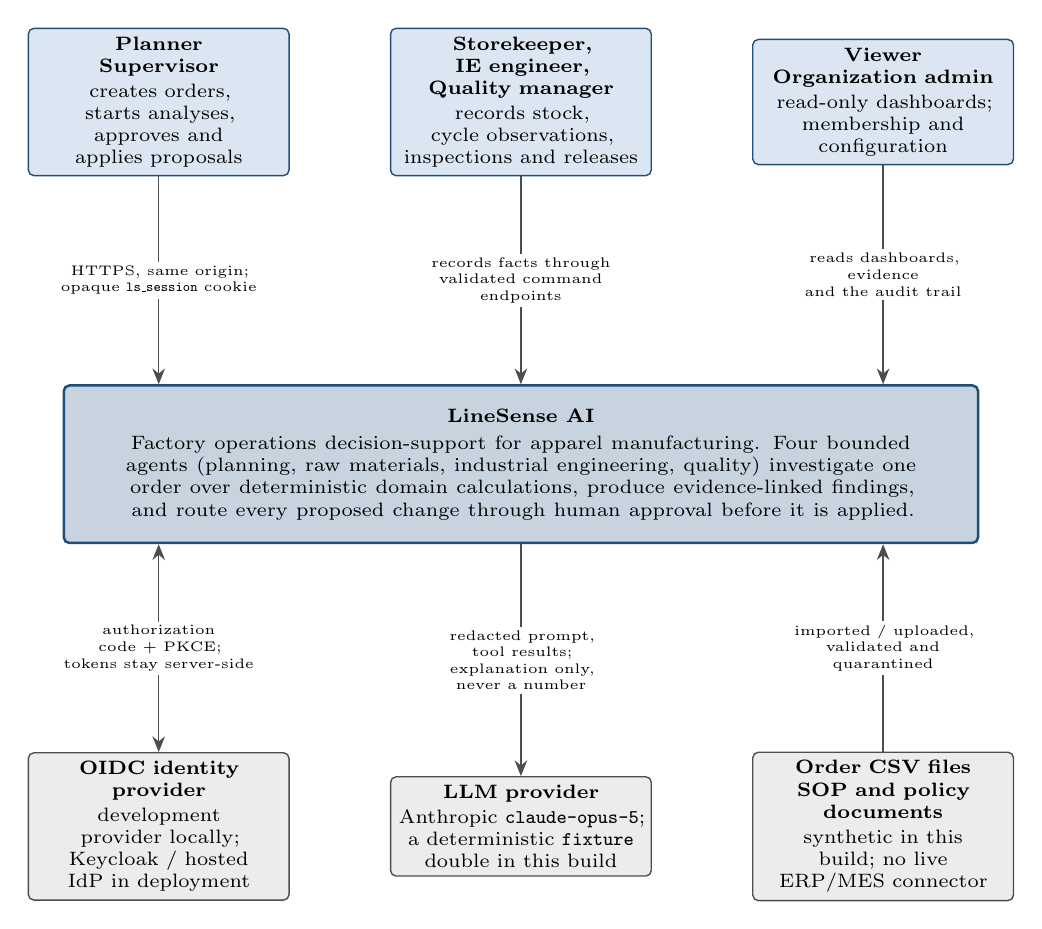
\begin{tikzpicture}

  % ---------- actors (row y = 4.6) -------------------------------------
  \node[person, text width=3.1cm] (p1) at (-4.6, 4.6)
    {\textbf{Planner\\ Supervisor}\\[1pt]
     creates orders, starts analyses,\\ approves and applies proposals};
  \node[person, text width=3.1cm] (p2) at ( 0.0, 4.6)
    {\textbf{Storekeeper, IE engineer,\\ Quality manager}\\[1pt]
     records stock, cycle observations,\\ inspections and releases};
  \node[person, text width=3.1cm] (p3) at ( 4.6, 4.6)
    {\textbf{Viewer\\ Organization admin}\\[1pt]
     read-only dashboards;\\ membership and configuration};

  % ---------- the system (row y = 0) -----------------------------------
  \node[system, text width=11.4cm, minimum height=2.0cm] (sys) at (0,0)
    {LineSense AI\\[2pt]
     \normalfont\scriptsize Factory operations decision-support for apparel
     manufacturing. Four bounded agents (planning, raw materials, industrial
     engineering, quality) investigate one order over deterministic domain
     calculations, produce evidence-linked findings, and route every proposed
     change through human approval before it is applied.};

  % ---------- external systems (row y = -4.6) --------------------------
  \node[external, text width=3.1cm] (idp) at (-4.6,-4.6)
    {\textbf{OIDC identity provider}\\[1pt]
     development provider locally;\\ Keycloak / hosted IdP in deployment};
  \node[external, text width=3.1cm] (llm) at ( 0.0,-4.6)
    {\textbf{LLM provider}\\[1pt]
     Anthropic \texttt{claude-opus-5};\\
     a deterministic \texttt{fixture} double in this build};
  \node[external, text width=3.1cm] (src) at ( 4.6,-4.6)
    {\textbf{Order CSV files\\ SOP and policy documents}\\[1pt]
     synthetic in this build; no live ERP/MES connector};

  % ---------- connectors: actors -> system -----------------------------
  \draw[flow] (p1.south) -- node[lblw, midway]
      {HTTPS, same origin;\\ opaque \texttt{ls\_session} cookie}
      (p1.south |- sys.north);
  \draw[flow] (p2.south) -- node[lblw, midway]
      {records facts through\\ validated command endpoints}
      (p2.south |- sys.north);
  \draw[flow] (p3.south) -- node[lblw, midway]
      {reads dashboards, evidence\\ and the audit trail}
      (p3.south |- sys.north);

  % ---------- connectors: system -> external systems -------------------
  \draw[biflow] (idp.north |- sys.south) -- node[lblw, midway]
      {authorization code + PKCE;\\ tokens stay server-side}
      (idp.north);
  \draw[flow] (llm.north |- sys.south) -- node[lblw, midway]
      {redacted prompt, tool results;\\ explanation only, never a number}
      (llm.north);
  \draw[flow] (src.north) -- node[lblw, midway]
      {imported / uploaded,\\ validated and quarantined}
      (src.north |- sys.south);

\end{tikzpicture}
}
\caption{C4 level 1 --- system context. The three actor groups, the system, and
the three external systems it depends on. The LLM provider is drawn because the
boundary exists and is implemented; in this build it is always the deterministic
\texttt{fixture} double.}
\label{fig:context}
\end{figure}

\begin{figure}[p]
\centering
\resizebox{\textwidth}{!}{% C4 level 2 -- containers.
% Explicit grid.  Columns: x = -5.6 | 0 | 5.6.  Rows: y = 5.4 | 2.6 | -3.0 | -6.4.
% The band around y = -1.1 and the band at y = -5.0 are deliberately empty:
% they are the horizontal routing corridors used by the worker connectors.
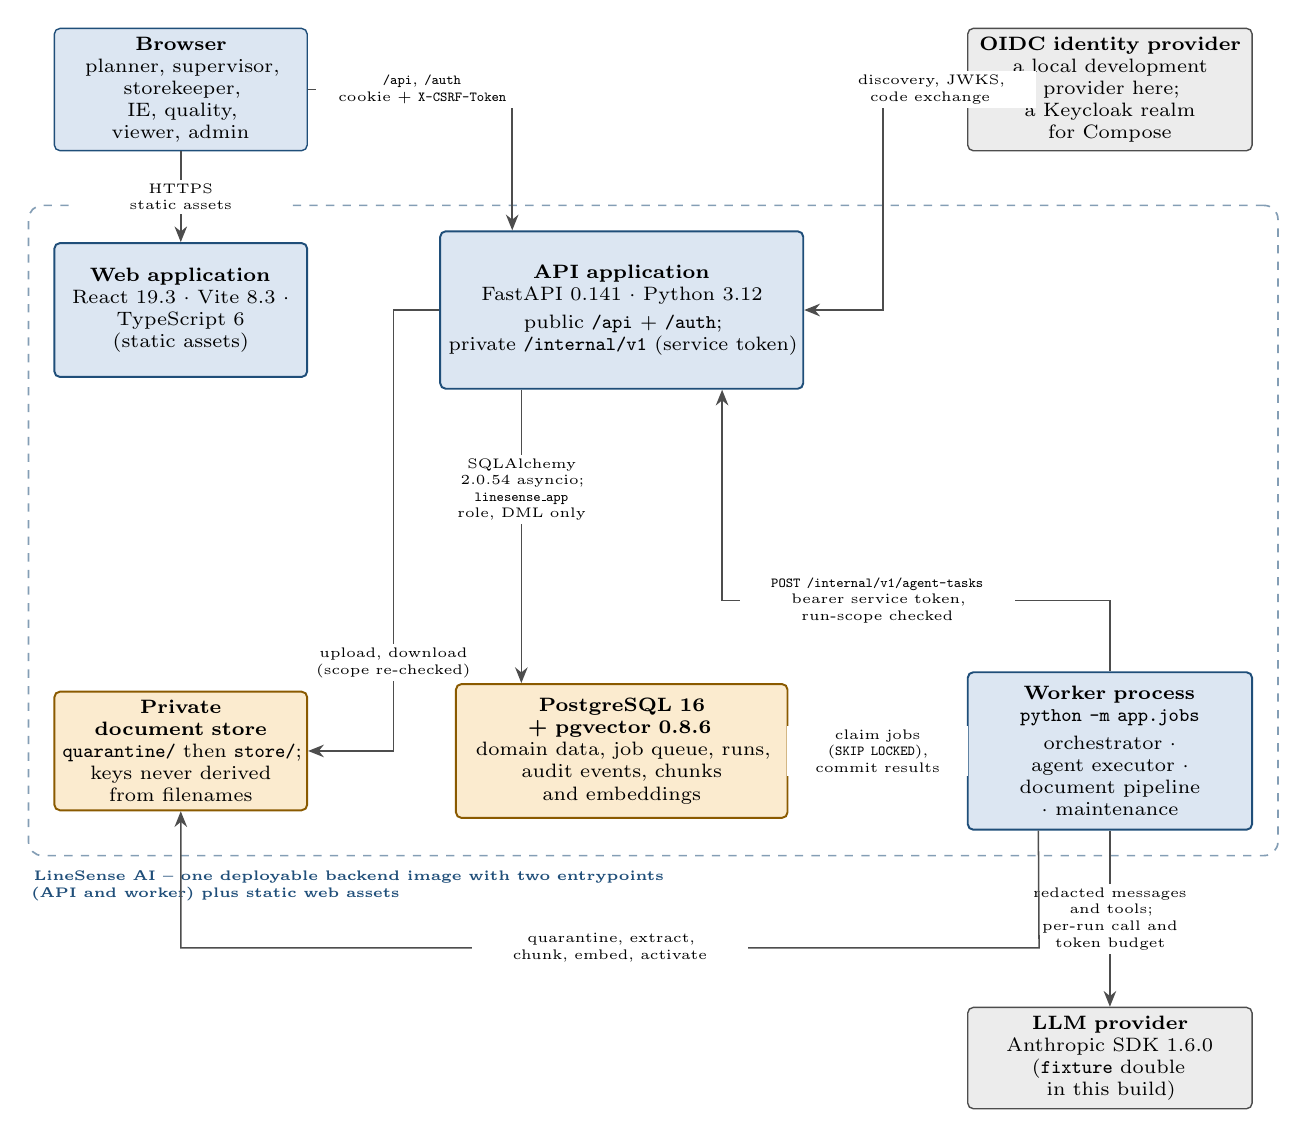
\begin{tikzpicture}

  % ---------- outside the system boundary ------------------------------
  \node[person,   text width=3.0cm] (browser) at (-5.6, 5.4)
    {\textbf{Browser}\\ planner, supervisor, storekeeper,\\ IE, quality, viewer, admin};
  \node[external, text width=3.4cm] (idp)     at ( 6.2, 5.4)
    {\textbf{OIDC identity provider}\\ a local development provider here;\\
     a Keycloak realm for Compose};
  \node[external, text width=3.4cm] (llm)     at ( 6.2,-6.9)
    {\textbf{LLM provider}\\ Anthropic SDK 1.6.0\\ (\texttt{fixture} double in this build)};

  % ---------- containers ------------------------------------------------
  \node[container, text width=3.0cm, minimum height=1.7cm] (web) at (-5.6, 2.6)
    {\textbf{Web application}\\ React 19.3 $\cdot$ Vite 8.3 $\cdot$\\ TypeScript 6\\ (static assets)};
  \node[container, text width=4.4cm, minimum height=2.0cm] (api) at ( 0.0, 2.6)
    {\textbf{API application}\\ FastAPI 0.141 $\cdot$ Python 3.12\\[2pt]
     \normalfont\scriptsize public \texttt{/api} + \texttt{/auth};\\
     private \texttt{/internal/v1} (service token)};
  \node[container, text width=3.4cm, minimum height=2.0cm] (worker) at ( 6.2,-3.0)
    {\textbf{Worker process}\\ \texttt{python -m app.jobs}\\[2pt]
     \normalfont\scriptsize orchestrator $\cdot$ agent executor $\cdot$\\
     document pipeline $\cdot$ maintenance};
  \node[store, text width=4.0cm, minimum height=1.7cm] (db) at ( 0.0,-3.0)
    {\textbf{PostgreSQL 16 + pgvector 0.8.6}\\ domain data, job queue, runs,\\
     audit events, chunks and embeddings};
  \node[store, text width=3.0cm, minimum height=1.5cm] (docs) at (-5.6,-3.0)
    {\textbf{Private document store}\\ \texttt{quarantine/} then \texttt{store/};\\
     keys never derived from filenames};

  % system boundary
  \begin{scope}[on background layer]
    \node[boundary, fit=(web)(api)(worker)(db)(docs)] (bnd) {};
  \end{scope}
  \node[boundlbl, anchor=north west, text width=8.0cm]
    at ([shift={(0pt,-3pt)}]bnd.south west)
    {LineSense AI -- one deployable backend image with two entrypoints
     (API and worker) plus static web assets};

  % helper anchors so two connectors never share one edge point
  \coordinate (apiNl) at ($(api.north)!0.60!(api.north west)$);
  \coordinate (apiSl) at ($(api.south)!0.55!(api.south west)$);
  \coordinate (apiSr) at ($(api.south)!0.55!(api.south east)$);
  \coordinate (wkSl)  at ($(worker.south)!0.50!(worker.south west)$);

  % ---------- connectors -------------------------------------------------
  % browser -> static assets (pure vertical)
  \draw[flow] (browser.south) -- node[lblw, midway]
      {HTTPS\\ static assets} (browser.south |- web.north);

  % browser -> API : horizontal along y = 5.4, then vertical down into the API
  \draw[flow] (browser.east) -| node[lblw, pos=0.28]
      {\texttt{/api}, \texttt{/auth}\\ cookie + \texttt{X-CSRF-Token}} (apiNl);

  % API <-> identity provider : vertical at x = 3.3, then horizontal
  \draw[biflow] (api.east) -- ++(1.0,0)
      |- node[lblw, pos=0.78] {discovery, JWKS,\\ code exchange} (idp.west);

  % API -> database (pure vertical, left half of the API box)
  \draw[flow] (apiSl) -- node[lblw, pos=0.34]
      {SQLAlchemy 2.0.54 asyncio;\\ \texttt{linesense\_app} role, DML only}
      (apiSl |- db.north);

  % worker -> internal dispatch : up, along the empty corridor y = -1.1, then up
  \draw[flow] (worker.north) -- ++(0,0.9)
      -| node[lblx, pos=0.30]
        {\texttt{POST /internal/v1/agent-tasks}\\ bearer service token, run-scope checked}
      (apiSr);

  % worker <-> database
  \draw[biflow] (worker.west) -- node[lbl, midway, text width=2.2cm]
      {claim jobs\\ (\texttt{SKIP LOCKED}),\\ commit results} (db.east);

  % worker -> LLM provider (pure vertical)
  \draw[flow] (worker.south) -- node[lblw, midway]
      {redacted messages and tools;\\ per-run call and token budget}
      (worker.south |- llm.north);

  % API -> document store : left corridor at x = -2.9
  \draw[flow] (api.west) -- (-2.9, 2.6)
      -- node[lblw, pos=0.80] {upload, download\\ (scope re-checked)} (-2.9,-3.0)
      -- (docs.east);

  % worker -> document store : corridor below the database row, y = -5.0
  \coordinate (wkDown) at (5.3,-5.5);
  \draw[flow] (wkSl) -- (wkDown)
      -- node[lblx, midway] {quarantine, extract, chunk, embed, activate}
         (-5.6,-5.5) -- (docs.south);

\end{tikzpicture}
}
\caption{C4 level 2 --- containers. \texttt{API} and the internal dispatch
endpoint are the \emph{same} application with a public and a private routing
boundary; the worker is the same deployable image with a different entrypoint.
The browser can reach neither the database, nor the provider key, nor
\texttt{/internal/v1}.}
\label{fig:container}
\end{figure}

\begin{figure}[p]
\centering
\resizebox{\textwidth}{!}{% Component view of the backend (C4 level 3, collapsed to its dependency
% layers).  Layers are stacked wide boxes on a fixed vertical grid; every
% connector between adjacent layers is a pure vertical segment, and the two
% connectors that skip a layer use the left (x = -7.1) and right (x = 7.1)
% routing corridors, outside every box.
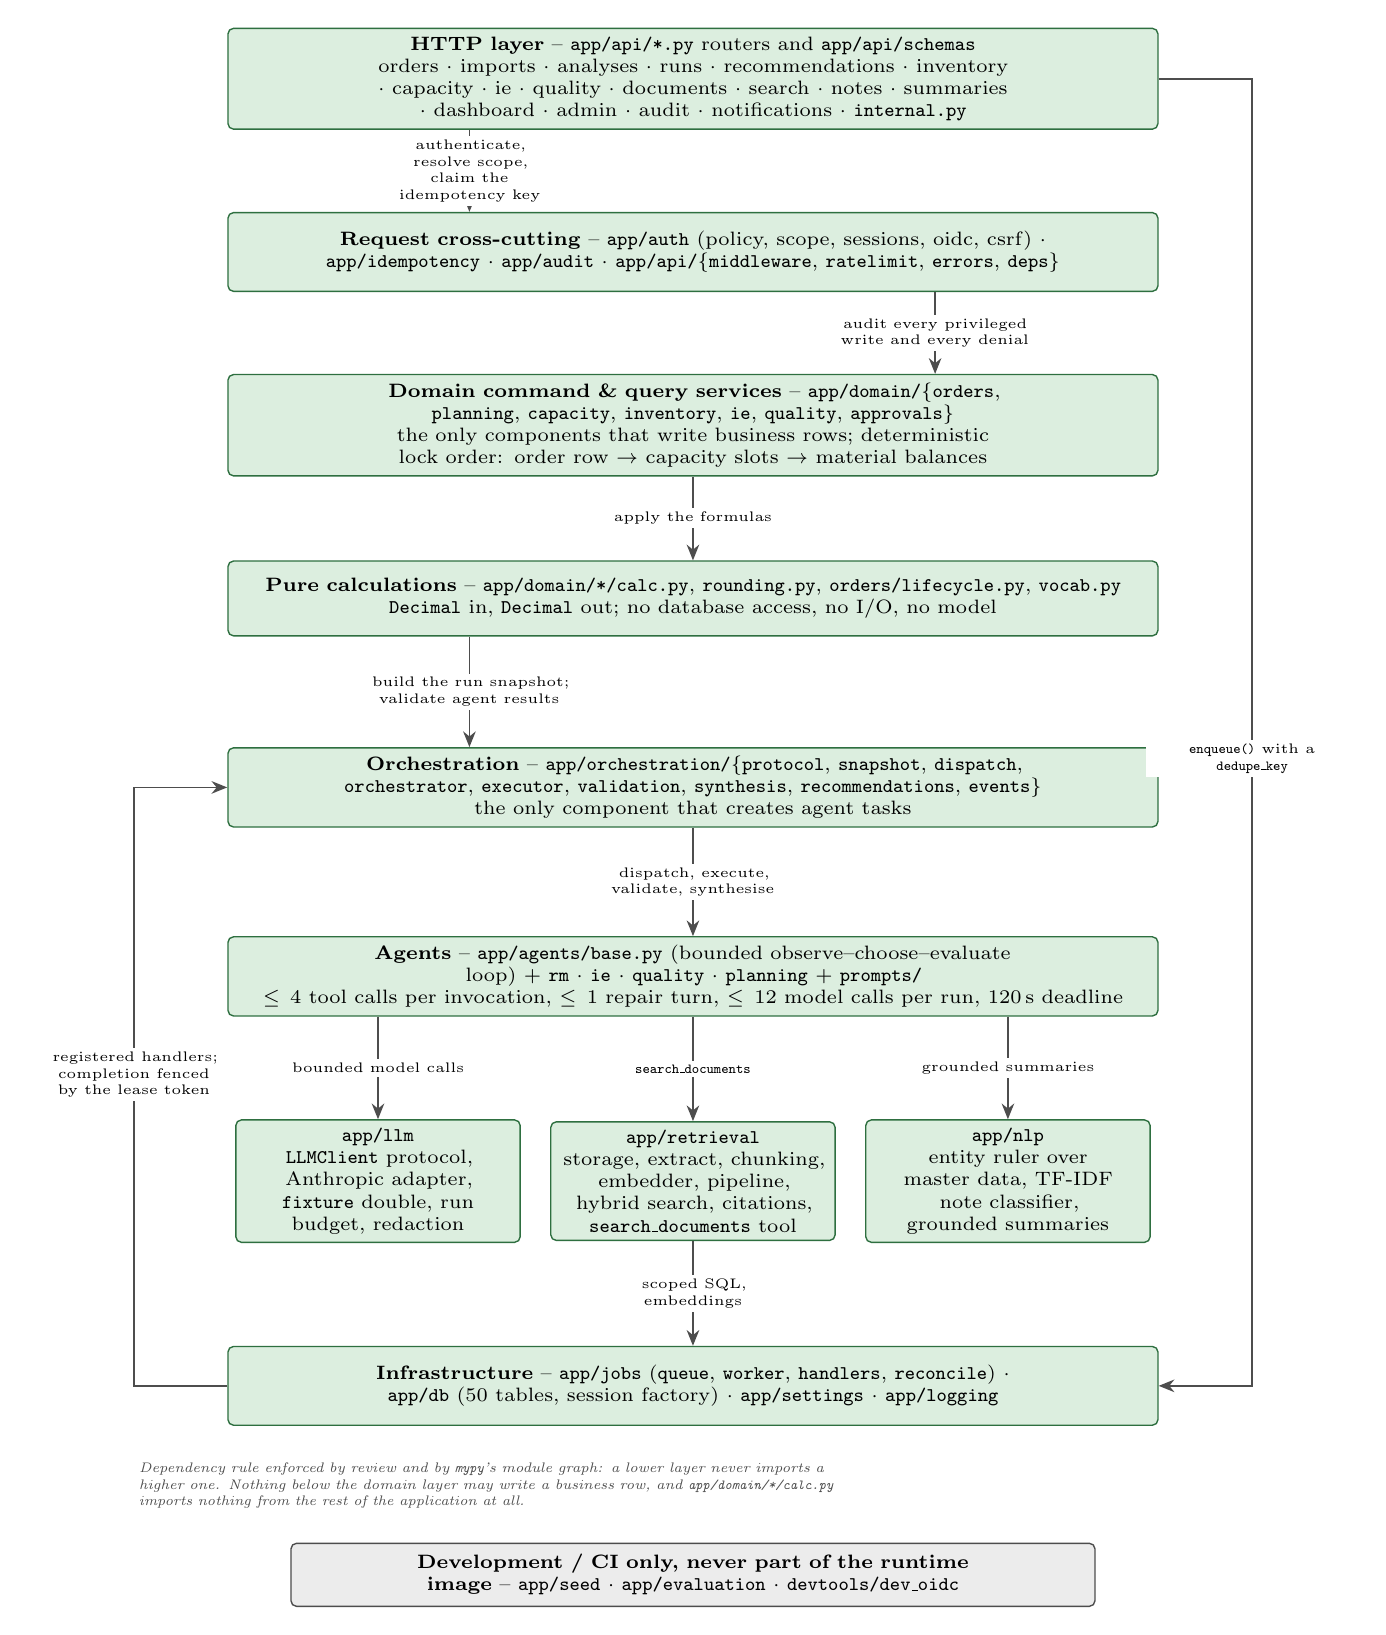
\begin{tikzpicture}[every node/.style={font=\scriptsize}]

  \def\W{11.6cm}

  \node[component, text width=\W, minimum height=1.05cm] (http)  at (0, 6.4)
    {\textbf{HTTP layer} -- \texttt{app/api/*.py} routers and \texttt{app/api/schemas}\\
     \normalfont\scriptsize orders $\cdot$ imports $\cdot$ analyses $\cdot$ runs $\cdot$ recommendations $\cdot$
     inventory $\cdot$ capacity $\cdot$ ie $\cdot$ quality $\cdot$ documents $\cdot$ search $\cdot$ notes $\cdot$
     summaries $\cdot$ dashboard $\cdot$ admin $\cdot$ audit $\cdot$ notifications $\cdot$ \texttt{internal.py}};

  \node[component, text width=\W, minimum height=1.0cm] (cross) at (0, 4.2)
    {\textbf{Request cross-cutting} -- \texttt{app/auth} (policy, scope, sessions, oidc, csrf) $\cdot$
     \texttt{app/idempotency} $\cdot$ \texttt{app/audit} $\cdot$ \texttt{app/api/}\{\texttt{middleware},
     \texttt{ratelimit}, \texttt{errors}, \texttt{deps}\}};

  \node[component, text width=\W, minimum height=1.0cm] (svc)   at (0, 2.0)
    {\textbf{Domain command \& query services} --
     \texttt{app/domain/}\{\texttt{orders}, \texttt{planning}, \texttt{capacity},
     \texttt{inventory}, \texttt{ie}, \texttt{quality}, \texttt{approvals}\}\\
     \normalfont\scriptsize the only components that write business rows; deterministic
     lock order: order row $\rightarrow$ capacity slots $\rightarrow$ material balances};

  \node[component, text width=\W, minimum height=0.95cm] (calc)  at (0,-0.2)
    {\textbf{Pure calculations} -- \texttt{app/domain/*/calc.py},
     \texttt{rounding.py}, \texttt{orders/lifecycle.py}, \texttt{vocab.py}\\
     \normalfont\scriptsize \texttt{Decimal} in, \texttt{Decimal} out; no database access, no I/O, no model};

  \node[component, text width=\W, minimum height=1.0cm] (orch)  at (0,-2.6)
    {\textbf{Orchestration} -- \texttt{app/orchestration/}\{\texttt{protocol},
     \texttt{snapshot}, \texttt{dispatch}, \texttt{orchestrator}, \texttt{executor},
     \texttt{validation}, \texttt{synthesis}, \texttt{recommendations}, \texttt{events}\}\\
     \normalfont\scriptsize the only component that creates agent tasks};

  \node[component, text width=\W, minimum height=1.0cm] (agents) at (0,-5.0)
    {\textbf{Agents} -- \texttt{app/agents/base.py} (bounded observe--choose--evaluate loop)
     + \texttt{rm} $\cdot$ \texttt{ie} $\cdot$ \texttt{quality} $\cdot$ \texttt{planning} + \texttt{prompts/}\\
     \normalfont\scriptsize $\le 4$ tool calls per invocation, $\le 1$ repair turn,
     $\le 12$ model calls per run, 120\,s deadline};

  \node[component, text width=3.4cm, minimum height=1.35cm] (llm)  at (-4.0,-7.6)
    {\textbf{\texttt{app/llm}}\\ \normalfont\scriptsize \texttt{LLMClient} protocol,
     Anthropic adapter, \texttt{fixture} double, run budget, redaction};
  \node[component, text width=3.4cm, minimum height=1.35cm] (retr) at ( 0.0,-7.6)
    {\textbf{\texttt{app/retrieval}}\\ \normalfont\scriptsize storage, extract, chunking,
     embedder, pipeline, hybrid search, citations, \texttt{search\_documents} tool};
  \node[component, text width=3.4cm, minimum height=1.35cm] (nlp)  at ( 4.0,-7.6)
    {\textbf{\texttt{app/nlp}}\\ \normalfont\scriptsize entity ruler over master data,
     TF-IDF note classifier, grounded summaries};

  \node[component, text width=\W, minimum height=1.0cm] (infra) at (0,-10.2)
    {\textbf{Infrastructure} -- \texttt{app/jobs} (\texttt{queue}, \texttt{worker},
     \texttt{handlers}, \texttt{reconcile}) $\cdot$ \texttt{app/db} (50 tables, session factory) $\cdot$
     \texttt{app/settings} $\cdot$ \texttt{app/logging}};

  \node[external, text width=10.0cm, minimum height=0.8cm] (dev) at (0,-12.6)
    {\textbf{Development / CI only, never part of the runtime image} --
     \texttt{app/seed} $\cdot$ \texttt{app/evaluation} $\cdot$ \texttt{devtools/dev\_oidc}};

  % ---- adjacent-layer connectors (pure vertical, anchored on the boxes) --
  \coordinate (cA) at ($(http.south west)!0.26!(http.south east)$);
  \coordinate (cB) at ($(cross.south west)!0.76!(cross.south east)$);
  \coordinate (cC) at ($(svc.south west)!0.50!(svc.south east)$);
  \coordinate (cD) at ($(calc.south west)!0.26!(calc.south east)$);
  \coordinate (cE) at ($(orch.south west)!0.50!(orch.south east)$);

  \draw[flow] (cA) -- node[lblw, midway]
      {authenticate, resolve scope,\\ claim the idempotency key} (cA |- cross.north);
  \draw[flow] (cB) -- node[lblw, midway]
      {audit every privileged\\ write and every denial} (cB |- svc.north);
  \draw[flow] (cC) -- node[lblw, midway]
      {apply the formulas} (cC |- calc.north);
  \draw[flow] (cD) -- node[lblw, midway]
      {build the run snapshot;\\ validate agent results} (cD |- orch.north);
  \draw[flow] (cE) -- node[lblw, midway]
      {dispatch, execute,\\ validate, synthesise} (cE |- agents.north);
  \draw[flow] (llm.north  |- agents.south) -- node[lblw, midway] {bounded model calls} (llm.north);
  \draw[flow] (retr.north |- agents.south) -- node[lblw, midway] {\texttt{search\_documents}} (retr.north);
  \draw[flow] (nlp.north  |- agents.south) -- node[lblw, midway] {grounded summaries} (nlp.north);
  \draw[flow] (retr.south) -- node[lblw, midway] {scoped SQL, embeddings}
      (retr.south |- infra.north);

  % ---- layer-skipping connectors, routed outside every box --------------
  % The HTTP layer enqueues jobs directly (analysis creation, document upload).
  \draw[flow] (http.east) -- (7.1, 6.4) -- node[lblw, pos=0.52]
      {\texttt{enqueue()} with a\\ \texttt{dedupe\_key}} (7.1,-10.2) -- (infra.east);
  % The worker runtime invokes the registered orchestration handlers.
  \draw[flow] (infra.west) -- (-7.1,-10.2) -- node[lblw, pos=0.52]
      {registered handlers;\\ completion fenced\\ by the lease token} (-7.1,-2.6) -- (orch.west);

  \node[note, anchor=north west, text width=9.0cm] at (-7.1,-11.1)
    {Dependency rule enforced by review and by \texttt{mypy}'s module graph: a lower
     layer never imports a higher one. Nothing below the domain layer may write a
     business row, and \texttt{app/domain/*/calc.py} imports nothing from the rest of
     the application at all.};

\end{tikzpicture}
}
\caption{Component view of the backend, collapsed to its dependency layers. The
rule a lower layer never imports a higher one is what keeps
\texttt{app/domain/*/calc.py} free of every other concern: those modules import
nothing from the rest of the application at all.}
\label{fig:components}
\end{figure}

\clearpage
\subsection{Boundaries that are actually enforced}

\begin{itemize}
\item The browser holds an \textbf{opaque session identifier} and nothing else
  --- no profile data, no provider tokens, no bearer token in
  \texttt{localStorage}. Provider tokens stay server-side after the OIDC code
  exchange.
\item \texttt{/internal/v1} is excluded from the public OpenAPI document
  (\texttt{include\_in\_schema=False}), requires a constant-time-compared bearer
  service token, and is returned as \texttt{404} at the edge by the reverse
  proxy as an independent control.
\item Agents receive \textbf{read/compute tools over an immutable run snapshot}.
  No agent tool accepts SQL, a shell command or a URL; no tool can create
  another tool; and the tool set of each agent is fixed in code, never derived
  from request input.
\item Only the domain command services write business rows, and they do so under
  a single documented lock order: order row $\rightarrow$ recommendation row
  $\rightarrow$ capacity slots (ascending id) $\rightarrow$ material balances
  (ascending id).
\end{itemize}

\subsection{Data model}

The schema is 50 tables in one Alembic revision
(\texttt{migrations/versions/0001\_initial\_schema.py}), grouped as identity,
demand, capacity, inventory, IE, quality, documents, workflow, decisions and
operations. Every table uses UUID keys, explicit units, \texttt{Decimal}
quantities, UTC timestamps and a \texttt{version} column on mutable business
records.

Tenant safety is structural, not conventional. Tenant-owned rows carry
\texttt{organization\_id}; plant-specific rows also carry \texttt{factory\_id};
and every table with both \textbf{not null} uses a composite foreign key
\texttt{(organization\_id, factory\_id) $\rightarrow$ factories(organization\_id,
id)}, so a cross-organization factory reference is rejected by the database
itself. A dedicated integration test
(\texttt{test\_schema.py::test\_cross\_org\_factory\_reference\_rejected})
asserts this.

Three further schema-level guarantees worth naming:

\begin{itemize}
\item \texttt{audit\_events} has \textbf{no foreign keys at all} and the runtime
  role \texttt{linesense\_app} is granted \texttt{SELECT, INSERT} on it with
  \texttt{UPDATE, DELETE} revoked --- append-only at the privilege level, tested
  by \texttt{test\_app\_role\_cannot\_update\_or\_delete\_audit\_events}.
\item Inventory is a \textbf{ledger}. Receipts, issues and corrections are
  \texttt{stock\_movements} rows; a correction references the movement it
  corrects; and a lockable \texttt{material\_balances} row with its own
  \texttt{version} is the thing a transaction takes for update.
\item \texttt{chunks.tsv} is a persisted generated \texttt{TSVECTOR} column with
  a GIN index, and \texttt{chunks.embedding} is a
  \texttt{pgvector.sqlalchemy.Vector(384)} column --- lexical and vector search
  read the same row.
\end{itemize}

\subsection{State design}

Four separate state vocabularies are kept separate on purpose, because merging
them is exactly how a single misleading ``order status'' gets invented:

\begin{itemize}
\item \textbf{Production:} \texttt{DRAFT} $\rightarrow$ \texttt{VALIDATED}
  $\rightarrow$ \texttt{PLANNED} $\rightarrow$ \texttt{IN\_PRODUCTION}
  $\rightarrow$ \texttt{PRODUCTION\_COMPLETE} $\rightarrow$ \texttt{DISPATCHED},
  with explicit permitted cancellation transitions. Every transition is defined
  in one central policy table (\texttt{app/domain/orders/lifecycle.py}) with
  actor permissions, preconditions and audit requirements. \textbf{There is no
  \texttt{PATCH status} endpoint.}
\item \textbf{Materials:} \texttt{UNKNOWN} $|$ \texttt{READY} $|$
  \texttt{AT\_RISK} $|$ \texttt{SHORTAGE}.
\item \textbf{Quality:} \texttt{NOT\_INSPECTED} $|$ \texttt{PENDING} $|$
  \texttt{HOLD} $|$ \texttt{RELEASED}.
\item \textbf{Analysis (per run):} figure~\ref{fig:runstate}.
\end{itemize}

\texttt{shipment\_ready} is \emph{derived}, never stored as independent truth
and never selected by a model: production complete \textbf{and} the required
current inspections satisfied \textbf{and} no active hold \textbf{and}
packing/quantity records complete \textbf{and} an authorized quality release
recorded. Zero inspections yields \emph{unknown}, never \emph{pass}. A test
(\texttt{test\_a\_model\_all\_clear\_never\_makes\_the\_shipment\_eligible})
drives a scripted model that says ``All clear --- ready to ship'' and asserts
that neither the findings, the metric, nor \texttt{report.shipment.eligible}
change.

\begin{figure}[p]
\centering
\resizebox{\textwidth}{!}{% Orchestration state machine: the lifecycle of one analysis_runs row.
% The happy path is a vertical column at x = 0; the fan-out uses two dedicated
% vertical corridors (x = 2.2 and x = 2.8); cancellation and the deadline sweep
% use the left half.  Every connector is orthogonal and every edge label sits
% on a segment at least 2.2 cm long, so no label can reach a node.
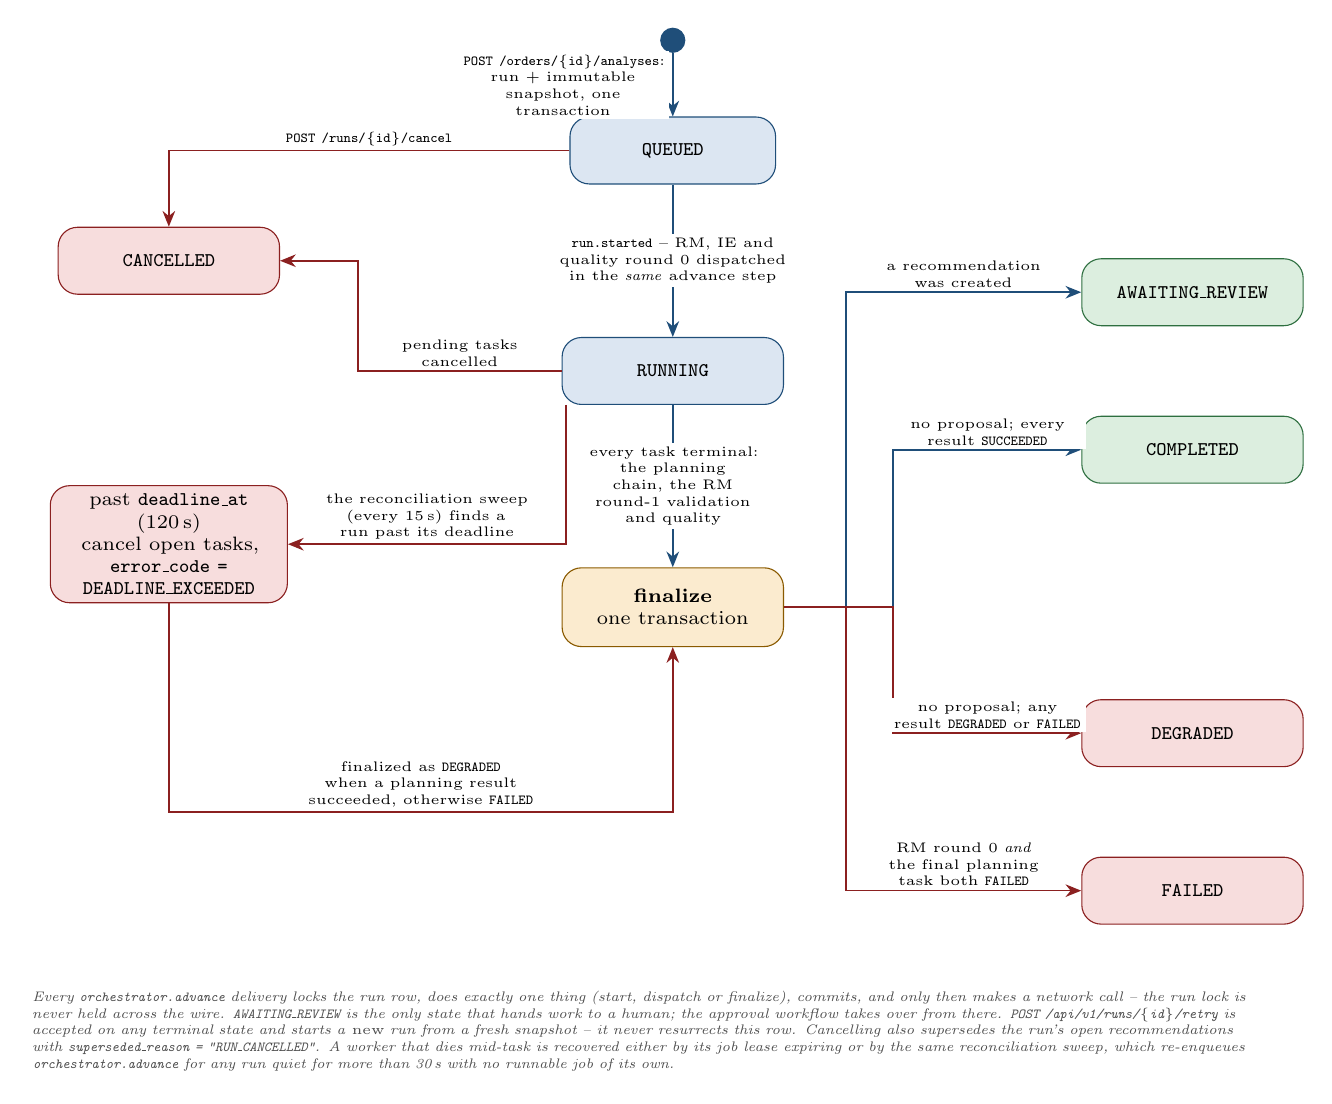
\begin{tikzpicture}[font=\scriptsize]

  % ---------- main column -------------------------------------------------
  \node[dot] (start) at (0, 6.4) {};
  \node[state, text width=2.4cm] (qu)  at (0, 5.0) {\texttt{QUEUED}};
  \node[state, text width=2.6cm] (run) at (0, 2.2) {\texttt{RUNNING}};
  \node[state, draw=lsamber, fill=lsamberd, text width=2.6cm, minimum height=1.0cm]
       (dec) at (0,-0.8) {\textbf{finalize}\\ one transaction};

  % ---------- terminal states (right column) ------------------------------
  \node[terminal, text width=2.6cm] (aw)   at (6.6, 3.2) {\texttt{AWAITING\_REVIEW}};
  \node[terminal, text width=2.6cm] (co)   at (6.6, 1.2) {\texttt{COMPLETED}};
  \node[badstate, text width=2.6cm] (deg)  at (6.6,-2.4) {\texttt{DEGRADED}};
  \node[badstate, text width=2.6cm] (fail) at (6.6,-4.4) {\texttt{FAILED}};

  % ---------- left column -------------------------------------------------
  \node[badstate, text width=2.6cm] (canc) at (-6.4, 3.6) {\texttt{CANCELLED}};
  \node[badstate, text width=2.8cm, minimum height=1.2cm] (dl) at (-6.4, 0.0)
      {past \texttt{deadline\_at} (120\,s)\\ \normalfont\scriptsize cancel open tasks,
       \texttt{error\_code = DEADLINE\_EXCEEDED}};

  % ---------- happy path --------------------------------------------------
  \draw[trans] (start) -- node[lbl, midway, text width=2.6cm, left=1pt]
      {\texttt{POST /orders/\{id\}/analyses}: run + immutable snapshot, one transaction}
      (qu.north);
  \draw[trans] (qu.south) -- node[lbl, midway, text width=3.4cm]
      {\texttt{run.started} -- RM, IE and quality round 0 dispatched in the
       \emph{same} advance step} (run.north);
  \draw[trans] (run.south) -- node[lbl, midway, text width=2.2cm]
      {every task terminal: the planning chain, the RM round-1 validation and
       quality} (dec.north);

  % ---------- fan-out -----------------------------------------------------
  \draw[trans] (dec.east) -- (2.2,-0.8) -- (2.2,3.2) --
      node[lbl, above, midway, text width=2.4cm] {a recommendation was created}
      (aw.west);
  \draw[trans] (dec.east) -- (2.8,-0.8) -- (2.8,1.2) --
      node[lbl, above, midway, text width=2.4cm]
      {no proposal; every result \texttt{SUCCEEDED}} (co.west);
  \draw[badtrans] (dec.east) -- (2.8,-0.8) -- (2.8,-2.4) --
      node[lbl, above, midway, text width=2.4cm]
      {no proposal; any result \texttt{DEGRADED} or \texttt{FAILED}} (deg.west);
  \draw[badtrans] (dec.east) -- (2.2,-0.8) -- (2.2,-4.4) --
      node[lbl, above, midway, text width=2.4cm]
      {RM round 0 \emph{and} the final planning task both \texttt{FAILED}}
      (fail.west);

  % ---------- cancellation ------------------------------------------------
  \draw[badtrans] (qu.west) -- node[lbl, above, midway, text width=2.8cm]
      {\texttt{POST /runs/\{id\}/cancel}} (-6.4,5.0) -- (canc.north);
  \draw[badtrans] (run.west) -- node[lbl, above, midway, text width=2.4cm]
      {pending tasks cancelled} (-4.0,2.2) -- (-4.0,3.6) -- (canc.east);

  % ---------- deadline sweep ----------------------------------------------
  \coordinate (rSw) at ($(run.south)!0.96!(run.south west)$);
  \draw[badtrans] (rSw) -- (rSw |- dl.east) --
      node[lbl, above, midway, text width=3.0cm]
      {the reconciliation sweep (every 15\,s) finds a run past its deadline}
      (dl.east);
  \draw[badtrans] (dl.south) -- (-6.4,-3.4) --
      node[lbl, above, midway, text width=3.4cm]
      {finalized as \texttt{DEGRADED} when a planning result succeeded,
       otherwise \texttt{FAILED}} (0,-3.4) -- (dec.south);

  \node[note, anchor=north west, text width=15.4cm] at (-8.2,-5.6)
    {Every \texttt{orchestrator.advance} delivery locks the run row, does exactly
     one thing (start, dispatch or finalize), commits, and only then makes a
     network call -- the run lock is never held across the wire.
     \texttt{AWAITING\_REVIEW} is the only state that hands work to a human; the
     approval workflow takes over from there.
     \texttt{POST /api/v1/runs/\{id\}/retry} is accepted on any terminal state and
     starts a \emph{new} run from a fresh snapshot -- it never resurrects this row.
     Cancelling also supersedes the run's open recommendations with
     \texttt{superseded\_reason = "RUN\_CANCELLED"}. A worker that dies mid-task is
     recovered either by its job lease expiring or by the same reconciliation
     sweep, which re-enqueues \texttt{orchestrator.advance} for any run quiet for
     more than 30\,s with no runnable job of its own.};

\end{tikzpicture}
}
\caption{The analysis-run state machine. The orchestrator is the only component
that creates agent tasks, and every delivery of \texttt{orchestrator.advance}
does exactly one thing before committing.}
\label{fig:runstate}
\end{figure}

\begin{figure}[p]
\centering
\resizebox{\textwidth}{!}{% Durable job / lease state machine (app/jobs/queue.py).
% Three states on one horizontal axis at y = 0 with gaps wide enough for their
% edge labels; terminal states stacked at x = 7.4; the retry path runs along
% the empty corridor y = -3.4 and the heartbeat self-transition is a
% rectangular loop above the LEASED state.
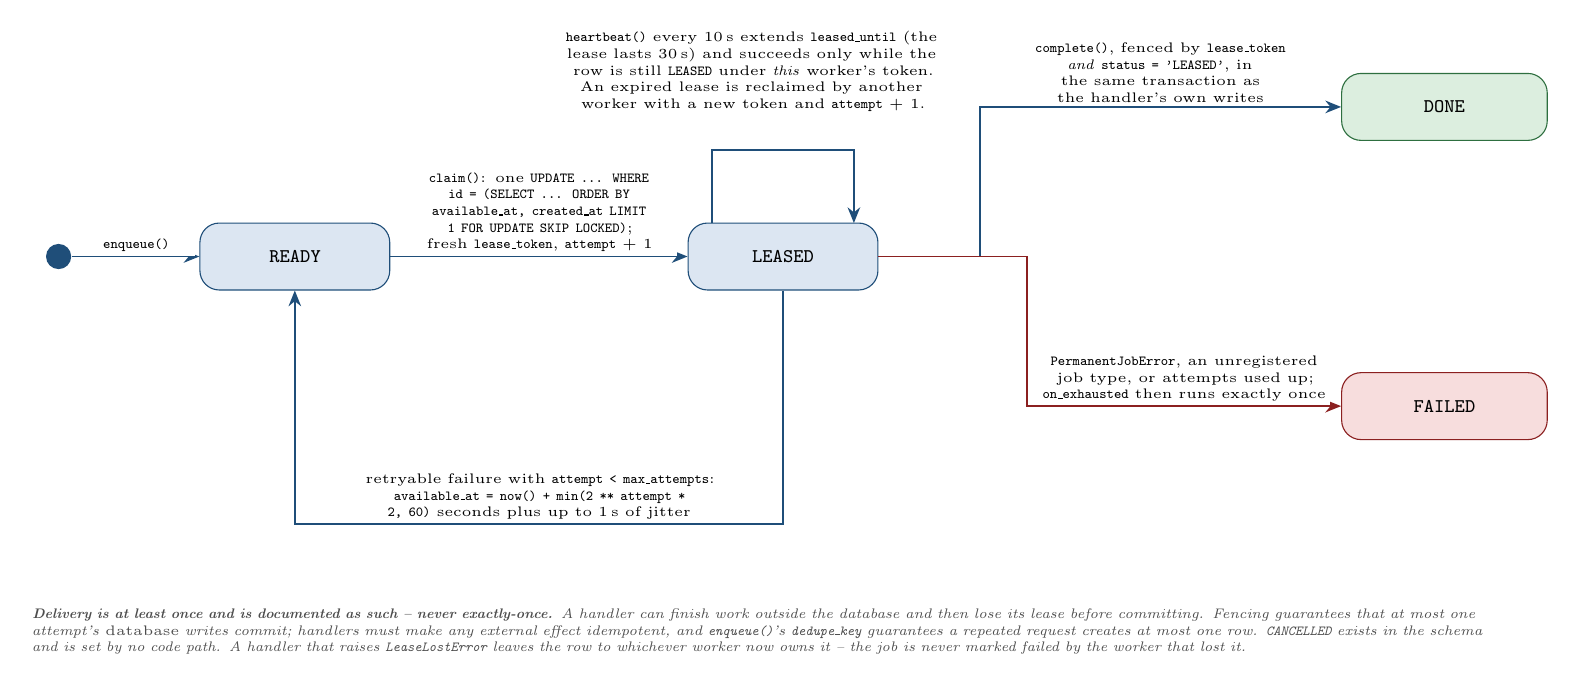
\begin{tikzpicture}[font=\scriptsize]

  \node[dot] (in) at (-10.2,0) {};
  \node[state, text width=2.2cm] (ready)  at (-7.2,0) {\texttt{READY}};
  \node[state, text width=2.2cm] (leased) at (-1.0,0) {\texttt{LEASED}};
  \node[terminal, text width=2.4cm] (done)   at (7.4, 1.9) {\texttt{DONE}};
  \node[badstate, text width=2.4cm] (failed) at (7.4,-1.9) {\texttt{FAILED}};

  \draw[trans] (in) -- node[lbl, above, midway, text width=1.4cm]
      {\texttt{enqueue()}} (ready.west);

  \draw[trans] (ready.east) -- node[lbl, above, midway, text width=3.4cm]
      {\texttt{claim()}: one \texttt{UPDATE ... WHERE id = (SELECT ... ORDER BY
       available\_at, created\_at LIMIT 1 FOR UPDATE SKIP LOCKED)}; fresh
       \texttt{lease\_token}, \texttt{attempt} + 1} (leased.west);

  % retry loop back to READY along the corridor y = -3.4
  \draw[trans] (leased.south) -- (-1.0,-3.4) --
      node[lbl, above, midway, text width=5.6cm]
      {retryable failure with \texttt{attempt < max\_attempts}:
       \texttt{available\_at = now() + min(2 ** attempt * 2, 60)} seconds plus up to
       1\,s of jitter} (-7.2,-3.4) -- (ready.south);

  % heartbeat / reclaim self-transition, above LEASED
  \draw[trans] (-1.9,0.425) -- (-1.9,1.35) -- (-0.1,1.35) -- (-0.1,0.425);
  \node[lbl, text width=5.6cm] at (-1.4,2.35)
      {\texttt{heartbeat()} every 10\,s extends \texttt{leased\_until} (the lease
       lasts 30\,s) and succeeds only while the row is still \texttt{LEASED} under
       \emph{this} worker's token. An expired lease is reclaimed by another worker
       with a new token and \texttt{attempt} + 1.};

  \draw[trans] (leased.east) -- (1.5,0) -- (1.5,1.9) --
      node[lbl, above, midway, text width=3.6cm]
      {\texttt{complete()}, fenced by \texttt{lease\_token} \emph{and}
       \texttt{status = 'LEASED'}, in the same transaction as the handler's own
       writes} (done.west);

  \draw[badtrans] (leased.east) -- (2.1,0) -- (2.1,-1.9) --
      node[lbl, above, midway, text width=3.6cm]
      {\texttt{PermanentJobError}, an unregistered job type, or attempts used up;
       \texttt{on\_exhausted} then runs exactly once} (failed.west);

  \node[note, anchor=north west, text width=18.4cm] at (-10.6,-4.4)
    {\textbf{Delivery is at least once and is documented as such -- never
     exactly-once.} A handler can finish work outside the database and then lose
     its lease before committing. Fencing guarantees that at most one attempt's
     \emph{database} writes commit; handlers must make any external effect
     idempotent, and \texttt{enqueue()}'s \texttt{dedupe\_key} guarantees a repeated
     request creates at most one row. \texttt{CANCELLED} exists in the schema and
     is set by no code path. A handler that raises \texttt{LeaseLostError} leaves
     the row to whichever worker now owns it -- the job is never marked failed by
     the worker that lost it.};

\end{tikzpicture}
}
\caption{The durable job and lease state machine. Delivery is at least once and
is documented as such; fencing by \texttt{lease\_token} guarantees that at most
one attempt's database writes commit.}
\label{fig:jobstate}
\end{figure}

\clearpage
% =====================================================================
\section{Technology stack and exact versions}
% =====================================================================

Versions below are the \textbf{locked} versions from
\texttt{services/backend/uv.lock} and \texttt{apps/web/package-lock.json} as
committed, not the version ranges in the manifests. The backend lock resolves
114 packages; the web lock resolves 419 entries. Third-party licences for every
one of them are inventoried in \texttt{docs/assessment/licenses.md}, generated
by \texttt{scripts/gen\_licenses.sh}.

\begin{table}[h]
\centering\small
\caption{Backend runtime dependencies (direct), locked versions. Python 3.12,
managed by \texttt{uv}.}
\begin{tabular}{@{}llL{7.6cm}@{}}
\toprule
\textbf{Package} & \textbf{Version} & \textbf{Role}\\
\midrule
\texttt{fastapi}          & 0.141.1 & HTTP API, dependency injection, OpenAPI generation\\
\texttt{starlette}        & 1.6.0   & ASGI foundation (transitive, pinned by the lock)\\
\texttt{uvicorn[standard]}& 0.53.0  & ASGI server (\texttt{api} entrypoint)\\
\texttt{pydantic}         & 2.13.5  & request/response models, the agent protocol models\\
\texttt{pydantic-settings}& 2.15.0  & \texttt{LS\_*} settings with a production hardening validator\\
\texttt{sqlalchemy[asyncio]} & 2.0.54 & ORM, async sessions, row locking\\
\texttt{alembic}          & 1.20.0  & migrations (one revision, 50 tables)\\
\texttt{psycopg[binary]}  & 3.3.5   & PostgreSQL driver\\
\texttt{pgvector}         & 0.5.0   & SQLAlchemy \texttt{Vector} column type\\
\texttt{authlib}          & 1.8.0   & OIDC client (authorization code + PKCE)\\
\texttt{joserfc}          & 1.7.5   & JOSE primitives used by the development IdP\\
\texttt{itsdangerous}     & 2.2.0   & signed handshake cookie for the OIDC state\\
\texttt{python-multipart} & 0.0.32  & multipart parsing for document upload\\
\texttt{httpx}            & 0.28.1  & internal dispatch client, test transport\\
\texttt{anthropic}        & 1.6.0   & LLM provider SDK (\emph{never called live in this build})\\
\texttt{structlog}        & 26.1.0  & JSON logging with trace ids and key redaction\\
\texttt{fastembed}        & 0.8.0   & ONNX embedding runtime (\texttt{BAAI/bge-small-en-v1.5}, 384 d)\\
\texttt{spacy}            & 3.8.16  & \texttt{blank("en")} + \texttt{EntityRuler} for entity extraction\\
\texttt{scikit-learn}     & 1.9.1   & TF-IDF + logistic regression note classifier\\
\texttt{numpy}            & 2.5.3   & vector arithmetic\\
\texttt{pypdf}            & 6.19.0  & PDF structural scan and text extraction\\
\texttt{pyyaml}           & 6.0.3   & dataset front matter, Compose/CI static validation\\
\bottomrule
\end{tabular}
\end{table}

\begin{table}[h]
\centering\small
\caption{Backend development dependencies and notable transitive runtime packages.}
\begin{tabular}{@{}llll@{}}
\toprule
\textbf{Dev package} & \textbf{Version} & \textbf{Transitive (notable)} & \textbf{Version}\\
\midrule
\texttt{pytest}        & 9.1.1  & \texttt{onnxruntime} & 1.30.0\\
\texttt{pytest-asyncio}& 1.4.0  & \texttt{tokenizers}  & 0.23.2\\
\texttt{hypothesis}    & 6.168.0& \texttt{huggingface-hub} & 1.31.0\\
\texttt{mypy}          & 2.3.1  & \texttt{scipy}       & 1.18.1\\
\texttt{ruff}          & 0.16.8 & \texttt{thinc}       & 8.3.13\\
\texttt{types-pyyaml}  & 6.0.12.20260906 & \texttt{cryptography} & 50.0.1\\
\bottomrule
\end{tabular}
\end{table}

\begin{table}[h]
\centering\small
\caption{Frontend dependencies, locked versions (\texttt{apps/web}). Node 26
(\texttt{.nvmrc}); TypeScript strict mode.}
\begin{tabular}{@{}llL{7.2cm}@{}}
\toprule
\textbf{Package} & \textbf{Version} & \textbf{Role}\\
\midrule
\texttt{react} / \texttt{react-dom} & 19.3.0 & UI runtime\\
\texttt{vite}              & 8.3.0   & dev server (proxying \texttt{/api}, \texttt{/auth}) and production build\\
\texttt{typescript}        & 6.0.3   & strict-mode types; \texttt{tsc -b} in CI\\
\texttt{react-router}      & 8.4.0   & data router, lazy route chunks\\
\texttt{@tanstack/react-query} & 5.103.1 & server state, explicit loading/error states, polling\\
\texttt{react-hook-form}   & 7.88.0  & forms\\
\texttt{@hookform/resolvers} & 5.9.1 & Zod resolver\\
\texttt{zod}               & 4.6.5   & client-side schemas mirroring the server contract\\
\texttt{openapi-fetch}     & 0.17.0  & typed client over the generated API types\\
\texttt{openapi-typescript}& 7.13.0  & generates \texttt{src/generated/api.ts} from \texttt{contracts/openapi.json}\\
\texttt{tailwindcss} / \texttt{@tailwindcss/vite} & 4.3.3 & CSS-first design tokens\\
\texttt{recharts}          & 3.10.1  & capacity, bottleneck and defect-trend charts\\
\texttt{@phosphor-icons/react} & 2.1.10 & icons (always paired with text)\\
\texttt{@fontsource-variable/geist} & 5.3.0 & self-hosted fonts (no third-party font CDN)\\
\texttt{vitest}            & 5.0.1   & component and unit tests\\
\texttt{@testing-library/react} & 16.3.3 & behaviour-focused component tests\\
\texttt{msw}               & 2.15.0  & request mocking in component tests\\
\texttt{jsdom}             & 30.1.0  & test DOM\\
\texttt{eslint}            & 10.11.0 & lint (\texttt{--max-warnings=0})\\
\bottomrule
\end{tabular}
\end{table}

\begin{table}[h]
\centering\small
\caption{Infrastructure and platform components. Container image tags were each
confirmed against the registry's own API before being pinned; none of these
images has ever been built or run here.}
\begin{tabular}{@{}lll@{}}
\toprule
\textbf{Component} & \textbf{Version / tag} & \textbf{Status in this build}\\
\midrule
PostgreSQL & 16.15 (Homebrew \texttt{postgresql@16}) & running locally, port 55432, project-local cluster\\
pgvector & 0.8.6 (compiled from source) & running locally (\texttt{CREATE EXTENSION vector})\\
Python & 3.12 & running locally\\
\texttt{uv} & 0.11.17 locally; \texttt{0.12.17} pinned in the image & running locally\\
Node.js & 26 (\texttt{apps/web/.nvmrc}) & running locally\\
\texttt{python} image & \texttt{3.12.14-slim-bookworm} & \textbf{never built}\\
\texttt{node} image & \texttt{26.9.0-alpine} & \textbf{never built}\\
\texttt{caddy} image & \texttt{2.11-alpine} & \textbf{never built}\\
\texttt{pgvector/pgvector} image & \texttt{0.8.6-pg16} & \textbf{never built}\\
\texttt{quay.io/keycloak/keycloak} & \texttt{26.7.4} & \textbf{never started}\\
GitHub Actions & \texttt{checkout@v7.0.1}, \texttt{setup-node@v7.0.0}, \texttt{setup-uv@v10.1.0}, \texttt{upload-artifact@v7.0.1} & workflow committed; not observed running\\
\bottomrule
\end{tabular}
\end{table}

\clearpage
% =====================================================================
\section{The four agents and bounded autonomy}
% =====================================================================

\subsection{The shape every agent has}

Every agent is the same shape (\texttt{app/agents/base.py}):

\begin{enumerate}
\item \texttt{assess(ctx)} runs first and is \textbf{deterministic}. It is the
  only source of findings, metrics, action payloads and evidence.
\item If no LLM client is configured, the result is returned immediately as
  \texttt{DEGRADED} with \texttt{degraded\_reason = "LLM\_DISABLED"} and the
  warning \emph{``AI explanation unavailable''}.
\item Otherwise a bounded loop runs: at most \textbf{4 investigative tool
  calls}, at most \textbf{1 repair turn}, and a hard iteration cap of
  $4+2+1$. \emph{Every} model call is reserved against the run's budget in the
  database \emph{before} it is made.
\item The first user message is JSON context inside
  \texttt{<context>\dots</context>} plus the instruction to treat tool results
  and documents as untrusted data and to select only among
  \texttt{candidate\_actions} and cite only \texttt{available\_evidence}. Tool
  output is redacted (\texttt{redact\_payload}) before it reaches the model.
\item \texttt{submit\_assessment} is validated server-side (action id, finding
  ids, evidence ids). One repair turn is offered; a second failure degrades the
  result to \texttt{INVALID\_AGENT\_OUTPUT} with the deterministic content
  intact.
\item On success the selected action moves to \texttt{rank=0} with its
  \textbf{payload unchanged}; the model's summary is used with
  \texttt{summary\_source="model"}; its notes become \texttt{MODEL\_NOTE}
  findings at severity \emph{info}.
\end{enumerate}

Run-wide limits: \textbf{12 model calls per run} shared by all six agent tasks,
\textbf{1 replan}, \textbf{2 retries} after the first attempt, and a
\textbf{120-second} deadline. The budget is reserved atomically
(\texttt{UPDATE analysis\_runs SET model\_calls\_used = model\_calls\_used + 1
WHERE \dots AND model\_calls\_used < model\_calls\_limit RETURNING \dots}), so
with a limit of 12, exactly 12 of any number of concurrent callers succeed ---
proved by a 30-way concurrent integration test.

\subsection{What each agent may and may not do}

\begin{table}[h]
\centering\small
\caption{The four agents (\texttt{docs/architecture/agents.md}).}
\begin{tabularx}{\linewidth}{@{}L{1.5cm}YL{4.1cm}@{}}
\toprule
\textbf{Agent} & \textbf{Deterministic assessment and tools} & \textbf{Human boundary}\\
\midrule
\texttt{rm} &
\texttt{assess\_material\_readiness} (r0), \texttt{validate\_plan\_materials} (r1).
Applies \texttt{app.domain.inventory.calc} only: \texttt{gross\_demand},
\texttt{available\_now}, \texttt{shortage}, \texttt{projected\_balance},
\texttt{coverage\_days}, \texttt{reorder\_point}, \texttt{coverable\_units},
\texttt{material\_state}. Tools: \texttt{get\_material\_position},
\texttt{get\_expected\_receipts}, \texttt{get\_consumption\_history},
\texttt{get\_bom\_demand}, \texttt{search\_documents}. &
Suggests replenishment. \textbf{Never buys, never reserves, never approves.} A
\texttt{RESERVATION} action is a proposal a human approves.\\
\addlinespace
\texttt{ie} &
\texttt{assess\_line\_capability}. Per-operation representative cycle (median,
$\ge 3$ samples), effective cycle, bottleneck, this model's balance index,
SAM-based vs measured throughput. Tools: \texttt{get\_line\_analysis},
\texttt{get\_operation\_statistics} (count and median only),
\texttt{compare\_observed\_vs\_standard}, \texttt{search\_documents}. &
\textbf{Never judges, names, ranks or compares an individual worker.} Operator
aliases are not in the snapshot, no tool returns one, and no summary, finding or
action may contain one --- asserted in \texttt{tests/agents/test\_ie\_agent.py}.\\
\addlinespace
\texttt{quality} &
\texttt{assess\_quality\_status}. Defective rate and DHU reported
\emph{separately}; eligibility is the snapshot's calculated verdict, quoted
verbatim. Tools: \texttt{get\_inspections}, \texttt{get\_policy\_rules},
\texttt{get\_defect\_breakdown}, \texttt{search\_documents}. &
Never decides shipment readiness, never releases a hold. A defect belongs to an
operation and an inspection, \textbf{never to a person}.\\
\addlinespace
\texttt{planning} &
\texttt{propose\_allocation} (r0), \texttt{revise\_allocation} (r1). Every
candidate comes from \texttt{plan\_earliest\_slots}: \texttt{FULL\_EARLIEST},
\texttt{MATERIAL\_LIMITED} (capped at RM's \texttt{coverable\_units}),
\texttt{SINGLE\_LINE}, plus \texttt{SIMULATED} options. Tools:
\texttt{get\_dependency\_findings}, \texttt{list\_compatible\_lines},
\texttt{get\_remaining\_capacity}, \texttt{simulate\_allocation}. &
Proposes. The allocation takes effect only when a supervisor approves
\emph{and} applies the recommendation.\\
\bottomrule
\end{tabularx}
\end{table}

\subsection{Degradation is explicit, never a silent fallback}

\begin{table}[h]
\centering\small
\caption{What happens when the model path fails. In every case the findings,
metrics, actions and evidence are unchanged --- only the explanation is missing.}
\begin{tabular}{@{}ll@{}}
\toprule
\textbf{Situation} & \textbf{Result}\\
\midrule
\texttt{LS\_LLM\_PROVIDER=disabled} & \texttt{DEGRADED}, deterministic summary, \texttt{degraded\_reason = LLM\_DISABLED}\\
Provider outage & three attempts, then the deterministic assessment, \texttt{PROVIDER\_UNAVAILABLE}\\
Run budget spent & the deterministic assessment, \texttt{BUDGET\_EXCEEDED}\\
Model refusal / invalid output twice & the deterministic assessment, \texttt{LLM\_REFUSAL} / \texttt{INVALID\_AGENT\_OUTPUT}\\
\bottomrule
\end{tabular}
\end{table}

The run still finalizes into a \texttt{run.report} whose
\texttt{degraded\_reasons} name exactly what was lost. \textbf{Fallback text is
never promoted as a real model run.}

\subsection{The agent task protocol}

The protocol is a \textbf{custom, versioned HTTP/JSON contract}
(\texttt{schema\_version "1.0"}). It is \emph{not} A2A and \emph{not} MCP, and
this report does not call it either.

\begin{table}[h]
\centering\small
\caption{\texttt{TaskEnvelope} --- what the server verifies, not what the JSON claims.}
\begin{tabularx}{\linewidth}{@{}L{4.1cm}Y@{}}
\toprule
\textbf{Field} & \textbf{Rule enforced server-side}\\
\midrule
\texttt{run\_id}, \texttt{organization\_id}, \texttt{factory\_id}, \texttt{order\_id}, \texttt{snapshot\_id} & must all equal the loaded run's own ids\\
\texttt{parent\_task\_id} & when set, must be a task of the same run\\
\texttt{sender} & always \texttt{"orchestrator"}: a task can never create a task\\
\texttt{recipient} / \texttt{task\_type} & the task type must be in \texttt{ALLOWED\_TASK\_TYPES[recipient]}\\
\texttt{idempotency\_key} & exactly \texttt{f"\{run\_id\}:\{recipient\}:\{snapshot\_id\}:round-\{round\}"}; a repeat returns \texttt{200} with the existing task\\
\texttt{round} & \texttt{0..1} --- at most one replan\\
\texttt{deadline\_at} & must be $\le$ the run's own deadline\\
\texttt{constraints} & \texttt{max\_tool\_calls} \texttt{0..4}; \texttt{read\_only} is \texttt{Literal[True]}\\
\bottomrule
\end{tabularx}
\end{table}

An \texttt{AgentResult} carries \texttt{status}, \texttt{summary} with its
\texttt{summary\_source}, \texttt{findings[]}, typed \texttt{metrics[]},
\texttt{recommended\_actions[]}, \texttt{evidence\_refs[]}, \texttt{warnings[]},
\texttt{input\_versions}, \texttt{data\_quality} and
\texttt{execution\_metadata} (provider, model, counts, \texttt{prompt\_version},
\texttt{degraded}, \texttt{degraded\_reason}, timings).
\texttt{app/orchestration/validation.py} rejects a result whose evidence does
not resolve, whose records fall outside the run's organization or factory, whose
document version is not \texttt{ACTIVE}/\texttt{SUPERSEDED}, or whose action
payload names a slot or balance that is not in the run snapshot. A rejected
result is replaced by a \texttt{FAILED} result with
\texttt{INVALID\_AGENT\_OUTPUT}: \textbf{the run continues, and the bad output is
never stored as truth}.

Error codes and their retryability are decided by the server, never by the
model:
\texttt{PROVIDER\_UNAVAILABLE} (the only retryable one),
\texttt{MISSING\_DATA},
\texttt{STALE\_INPUT},
\texttt{BUDGET\_EXCEEDED},
\texttt{INVALID\_AGENT\_OUTPUT},
\texttt{POLICY\_DENIED} and
\texttt{DEADLINE\_EXCEEDED}.

\subsection{The orchestration graph}

\texttt{orchestrator.advance} is the \textbf{only} component that creates agent
tasks. Every delivery locks the run row, does exactly one thing (start,
dispatch, or finalize), commits, and \emph{only then} makes a network call ---
the run lock is never held across the wire.

RM, IE and quality round 0 are dispatched in the \emph{same} advance step, as
three \texttt{task.dispatched} events with consecutive ids before any
\texttt{task.completed}: none depends on another. Planning round 0 waits for RM
\textbf{and} IE to be terminal and receives both results as input references.
Quality is independent of the planning chain but must be terminal before
finalization, because the order report cannot be written without its facts.

The replan rule is exact. \texttt{needs\_replan(planning\_result, rm\_result)}
returns a reason \emph{only} when the rank-0 \texttt{ALLOCATION} action commits
more units than the RM agent's \texttt{coverable\_units} metric:

\begin{quote}\footnotesize\ttfamily
MATERIAL\_SHORTAGE\_CONFLICT: selected plan\\ allocates <x> units but materials cover <y>
\end{quote}

\noindent The reason is recorded verbatim in the \texttt{orchestrator.replan}
run event. The revision task ranks the \texttt{MATERIAL\_LIMITED} option first
and adds a \texttt{REVISED\_FOR\_MATERIAL} warning quoting the allocated and
requested units, the shortage, and the first open receipt date. At most one
replan happens per run.

\widefig{d4-agent-sequence}{The end-to-end four-agent analysis run. Read it as
the answer to ``what actually happens when a planner presses \emph{Start
analysis}''. Note three things: the three round-0 dispatches leave in one advance
step; the replan is driven by a \emph{deterministic} comparison of two agents'
numbers, not by a model's opinion; and finalization is one transaction that
writes the proposal, the canonical report, the notification and the audit event
together.}{0.93}
\label{fig:seq}

\subsection{Deterministic engineering calculations}

These are the formulas the agents apply. They are demonstration formulas: an IE
or domain owner must validate the production assumptions before real use, and
units and assumptions appear next to every result on screen.

\textbf{Planning.}
\[
\text{required\_standard\_minutes} = \text{remaining\_units} \times \text{SAM}
\qquad
\text{utilization} = \frac{\text{allocated\_standard\_minutes}}{\text{available\_standard\_minutes}}
\]
where available standard minutes sum
$\text{available\_operator\_minutes\_per\_shift} \times
\text{planned\_efficiency\_fraction}$ over the eligible slots. Efficiency is
applied \emph{once}. Allocation is deterministic earliest-due-date with a
documented tie-break of \texttt{(slot\_date, shift\_code, str(line\_id))}; an
infeasible order stays unscheduled with a reason
(\texttt{NO\_COMPATIBLE\_LINE}, \texttt{INSUFFICIENT\_CAPACITY\_BEFORE\_DUE\_DATE},
\texttt{LIMITED\_BY\_MATERIAL}).

\textbf{Materials.}
\[
\text{available\_now} = \text{accepted\_on\_hand} - \text{active\_reservations}
\qquad
\text{gross\_demand} = \text{planned\_units} \times \text{BOM\_qty} \times (1 + \text{wastage})
\]
\[
\text{projected\_balance}(t) = \text{available\_now} + \text{eligible\_receipts}(t) - \text{new\_demand}(t)
\qquad
\text{reorder\_point} = \bar{c}\, L + \text{safety\_stock}
\]
Reservations already excluded from \texttt{available\_now} are never subtracted
twice. Missing or zero consumption yields an \emph{unknown} coverage indicator
with an explanation --- \texttt{coverage\_days} returns \texttt{None}, never a
misleading zero.

\textbf{IE.} For the sequential-operation model, an operation's effective cycle
is its representative single-operator seconds per unit divided by the number of
equivalently capable parallel operators; the bottleneck effective cycle is the
maximum; estimated line output is $3600 / c_{\text{bottleneck}}$ units per hour.
The balance index is
$\sum c_i / (n \cdot c_{\text{bottleneck}}) \times 100$ and is labelled as
\emph{this model's index}, not a universal industrial KPI.

\textbf{Quality.} \texttt{defective\_units / inspected\_units} and DHU
(\texttt{total\_defects / inspected\_units} $\times$ 100) are reported
\emph{separately}. Zero inspections means \emph{unknown}, not \emph{pass}. The
applicable policy is versioned and approved; the demo policy carries the label
\emph{``Demo policy --- not a certified AQL standard''} and the system never
claims certified AQL/ISO compliance.

\subsection{Independent reference fixtures}

Six reference cases were worked by hand \emph{before} the code existed
(\texttt{docs/architecture/formulas.md}) and are asserted verbatim in
\texttt{tests/unit/test\_reference\_fixtures.py} and, for the two
concurrency/staleness cases, in integration tests.

\begin{table}[h]
\centering\small
\caption{Reference fixtures and where each is proved.}
\begin{tabularx}{\linewidth}{@{}L{5.6cm}L{3.9cm}Y@{}}
\toprule
\textbf{Case} & \textbf{Expected} & \textbf{Proved by}\\
\midrule
1{,}000 units at SAM 12 min; 20 operators, 420 min each, 75\% efficiency &
demand 12{,}000 std min; one-shift capacity 6{,}300; does not fit &
\texttt{test\_reference\_fixtures.py}\\
1{,}500 accepted m, 400 reserved; demand 1{,}000 units @ 1.2 m + 5\% wastage &
available 1{,}100; demand 1{,}260; \textbf{shortage 160 m} &
\texttt{test\_reference\_fixtures.py}; reproduced end-to-end by the seeded \texttt{PO-DEMO-001}\\
Three sequential effective cycles 40 / 60 / 50 s &
bottleneck 60 s; 60 units/h; balance index $\approx$83.33\% &
\texttt{test\_reference\_fixtures.py}; \texttt{test\_seeded\_demo\_line\_reproduces\_op04\_bottleneck}\\
100 inspected, 7 defective, 12 defects &
7\% defective rate; DHU 12; disposition from the approved policy &
\texttt{test\_reference\_fixtures.py}\\
Two simultaneous reservations of 80 from 100 available &
at most one succeeds; the other gets a conflict/shortage &
\texttt{tests/integration/test\_reservation\_concurrency.py}\\
Proposal pinned to stock version 4; stock moves to 5 before apply &
application rejected as stale; approval cannot bypass reanalysis &
\texttt{test\_approvals.py::test\_apply\_rejects\_stale\_inputs\_and\_supersedes\_the\_recommendation}\\
\bottomrule
\end{tabularx}
\end{table}

% =====================================================================
\section{Methodology}
% =====================================================================

\subsection{Deterministic core plus bounded agents}

The methodological claim of this project is narrow and testable: \emph{an LLM
is useful for selecting among permitted investigative actions and for
explaining a result, and is unsafe as a source of business facts.} Everything
in the architecture follows from taking that seriously --- the pure calculation
layer that imports nothing, the candidate-action list the model may only
re-rank, the evidence id whitelist, the server-side validation of every
submission, and the source label on every rendered value.

The consequence, which is worth stating plainly, is that a model failure
degrades the product's \emph{explanation} and never its \emph{correctness}. A
provider outage costs the user a paragraph of prose, not a wrong shortage
figure.

\subsection{Retrieval}

Documents are retrieved with \textbf{hybrid search}: a lexical ranking
(\texttt{ts\_rank\_cd(tsv, websearch\_to\_tsquery('english', :q))}) and a vector
ranking (\texttt{embedding <=> :qvec}, cosine distance, exact scan) run under
the \emph{same} SQL filter --- organization, factory (or organization-wide),
document ACL, and \texttt{ACTIVE} version --- and are fused by reciprocal-rank
fusion, $\sum 1/(k + \text{rank})$ with $k = 60$, over each list's top 20, then
truncated to the top 6.

The filter runs \textbf{before} any content reaches a model, and
\texttt{get\_citation()} re-runs the whole scope and ACL check when a citation
is opened. A \texttt{SUPERSEDED} chunk is visible only when a \texttt{run\_id}
names a run in the caller's scope whose stored agent results actually cite that
chunk id --- never a blanket ``any superseded chunk once you know a run''.

\begin{figure}[p]
\centering
\resizebox{\textwidth}{!}{% Document ingestion pipeline and the retrieval path it feeds.
% Snake layout on a fixed grid: row 1 runs left-to-right at y = 2.6, row 2
% runs right-to-left at y = -1.4, and the single turn between them is a pure
% vertical segment at x = 6.0.  Rejection exits leave upward at y = 6.4.
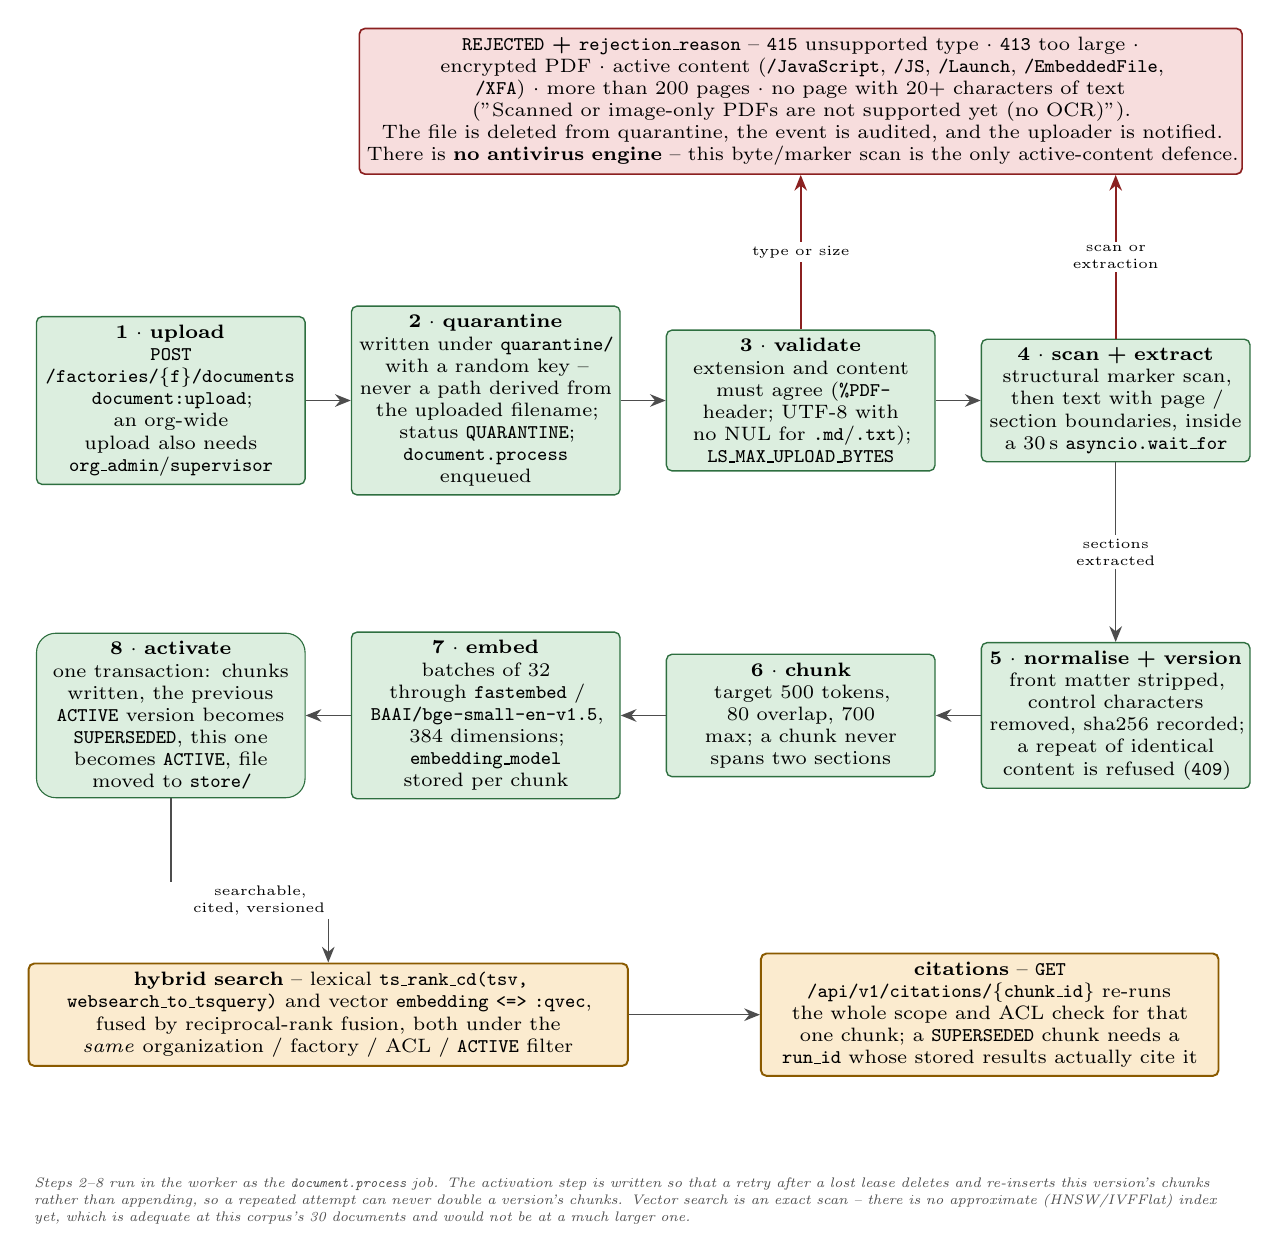
\begin{tikzpicture}[font=\scriptsize]

  % ---------- row 1 (left to right) --------------------------------------
  \node[component, text width=3.2cm, minimum height=1.5cm] (s1) at (-6.0, 2.6)
    {\textbf{1 $\cdot$ upload}\\ \texttt{POST /factories/\{f\}/documents}\\
     \normalfont\scriptsize \texttt{document:upload}; an org-wide upload also needs
     \texttt{org\_admin}/\texttt{supervisor}};
  \node[component, text width=3.2cm, minimum height=1.5cm] (s2) at (-2.0, 2.6)
    {\textbf{2 $\cdot$ quarantine}\\ \normalfont\scriptsize written under
     \texttt{quarantine/} with a random key -- never a path derived from the
     uploaded filename; status \texttt{QUARANTINE}; \texttt{document.process}
     enqueued};
  \node[component, text width=3.2cm, minimum height=1.5cm] (s3) at ( 2.0, 2.6)
    {\textbf{3 $\cdot$ validate}\\ \normalfont\scriptsize extension and content must agree
     (\texttt{\%PDF-} header; UTF-8 with no NUL for \texttt{.md}/\texttt{.txt});
     \texttt{LS\_MAX\_UPLOAD\_BYTES}};
  \node[component, text width=3.2cm, minimum height=1.5cm] (s4) at ( 6.0, 2.6)
    {\textbf{4 $\cdot$ scan + extract}\\ \normalfont\scriptsize structural marker scan, then
     text with page / section boundaries, inside a 30\,s
     \texttt{asyncio.wait\_for}};

  % ---------- row 2 (right to left) --------------------------------------
  \node[component, text width=3.2cm, minimum height=1.5cm] (s5) at ( 6.0,-1.4)
    {\textbf{5 $\cdot$ normalise + version}\\ \normalfont\scriptsize front matter stripped,
     control characters removed, sha256 recorded; a repeat of identical content is
     refused (\texttt{409})};
  \node[component, text width=3.2cm, minimum height=1.5cm] (s6) at ( 2.0,-1.4)
    {\textbf{6 $\cdot$ chunk}\\ \normalfont\scriptsize target 500 tokens, 80 overlap,
     700 max; a chunk never spans two sections};
  \node[component, text width=3.2cm, minimum height=1.5cm] (s7) at (-2.0,-1.4)
    {\textbf{7 $\cdot$ embed}\\ \normalfont\scriptsize batches of 32 through
     \texttt{fastembed} / \texttt{BAAI/bge-small-en-v1.5}, 384 dimensions;
     \texttt{embedding\_model} stored per chunk};
  \node[terminal, text width=3.2cm, minimum height=1.5cm] (s8) at (-6.0,-1.4)
    {\textbf{8 $\cdot$ activate}\\ \normalfont\scriptsize one transaction: chunks written,
     the previous \texttt{ACTIVE} version becomes \texttt{SUPERSEDED}, this one
     becomes \texttt{ACTIVE}, file moved to \texttt{store/}};

  % ---------- consumers ---------------------------------------------------
  \node[store, text width=7.4cm, minimum height=1.3cm] (search) at (-4.0,-5.2)
    {\textbf{hybrid search} -- lexical \texttt{ts\_rank\_cd(tsv,
     websearch\_to\_tsquery)} and vector \texttt{embedding <=> :qvec}, fused by
     reciprocal-rank fusion, both under the \emph{same} organization / factory /
     ACL / \texttt{ACTIVE} filter};
  \node[store, text width=5.6cm, minimum height=1.3cm] (cite) at ( 4.4,-5.2)
    {\textbf{citations} -- \texttt{GET /api/v1/citations/\{chunk\_id\}} re-runs the
     whole scope and ACL check for that one chunk; a \texttt{SUPERSEDED} chunk needs
     a \texttt{run\_id} whose stored results actually cite it};

  % ---------- rejection ---------------------------------------------------
  \node[danger, text width=11.0cm, minimum height=1.4cm] (rej) at (2.0, 6.4)
    {\textbf{\texttt{REJECTED} + \texttt{rejection\_reason}} -- \texttt{415}
     unsupported type $\cdot$ \texttt{413} too large $\cdot$ encrypted PDF $\cdot$ active content
     (\texttt{/JavaScript}, \texttt{/JS}, \texttt{/Launch}, \texttt{/EmbeddedFile},
     \texttt{/XFA}) $\cdot$ more than 200 pages $\cdot$ no page with 20+ characters of text
     ("Scanned or image-only PDFs are not supported yet (no OCR)").\\
     \normalfont\scriptsize The file is deleted from quarantine, the event is
     audited, and the uploader is notified. There is \textbf{no antivirus engine} --
     this byte/marker scan is the only active-content defence.};

  % ---------- connectors --------------------------------------------------
  \draw[flow] (s1.east) -- (s2.west);
  \draw[flow] (s2.east) -- (s3.west);
  \draw[flow] (s3.east) -- (s4.west);
  \draw[flow] (s4.south) -- node[lbl, midway, text width=1.9cm]
      {sections\\ extracted} (s5.north);
  \draw[flow] (s5.west) -- (s6.east);
  \draw[flow] (s6.west) -- (s7.east);
  \draw[flow] (s7.west) -- (s8.east);

  \draw[flow] (s8.south) -- ++(0,-1.3) -| node[lbl, pos=0.28, text width=2.4cm]
      {searchable, cited, versioned} (search.north);
  \draw[flow] (search.east) -- (cite.west);

  \draw[badtrans] (s3.north) -- node[lbl, midway, text width=1.8cm]
      {type or size} (s3.north |- rej.south);
  \draw[badtrans] (s4.north) -- node[lbl, midway, text width=1.8cm]
      {scan or extraction} (s4.north |- rej.south);

  \node[note, anchor=north west, text width=15.0cm] at (-7.8,-7.2)
    {Steps 2--8 run in the worker as the \texttt{document.process} job. The activation
     step is written so that a retry after a lost lease deletes and re-inserts this
     version's chunks rather than appending, so a repeated attempt can never double
     a version's chunks. Vector search is an exact scan -- there is no approximate
     (HNSW/IVFFlat) index yet, which is adequate at this corpus's 30 documents and
     would not be at a much larger one.};

\end{tikzpicture}
}
\caption{The document ingestion pipeline and the retrieval path it feeds.}
\label{fig:docs}
\end{figure}

\subsection{NLP}

Three capabilities, each deliberately starting from the simplest thing that
could work:

\begin{itemize}
\item \textbf{Entity extraction} is \texttt{spacy.blank("en")} plus one
  \texttt{EntityRuler} compiled from \emph{that factory's} authorized master
  data --- order refs, line codes and names, style codes, material codes and
  names, operation and defect codes and names. One extra token regex
  (\texttt{\^{}po-[a-z]\{3\}-\textbackslash d\{4\}\$}) surfaces well-formed but
  \emph{unknown} order references without ever resolving them. A BYG line code is
  not a pattern at all when the extractor is built for KTN, so it is not
  recognised --- not merely ``unresolved''. Ambiguity (two rows normalising to
  one key) yields a nil-UUID sentinel and the mention is dropped from both the
  resolved and unresolved lists: it is never stored and never actioned. The API
  always returns the notice \emph{``Entity links are for navigation only; they do
  not authorize any action.''}
\item \textbf{Note classification} has a documented keyword baseline and a
  \texttt{TfidfVectorizer(1,2-grams)} + \texttt{LogisticRegression} model
  trained \emph{only} from \texttt{data/eval/notes\_train.jsonl}. A unit test
  patches \texttt{builtins.open} to prove the test split is never opened during
  training. In production the classifier abstains (\texttt{"unknown"}) below a
  0.45 probability margin; the evaluation deliberately scores plain
  \texttt{.predict()} instead, because the margin is a product policy, not a
  measure of the model.
\item \textbf{Grounded summarization} computes a canonical structured report
  first and layers an optional model explanation second. Every sentence of the
  deterministic summary draws its evidence ids from the report's own blockers
  and evidence. The model path validates the response before using it: every
  sentence must carry evidence ids that exist, and no sentence matching
  \texttt{ready to ship|shipment[- ]ready|can ship} is accepted while
  \texttt{shipment.eligible} is false. Any failure falls back to the
  deterministic summary \emph{with a label saying why}.
\end{itemize}

\subsection{Evaluation design}

\texttt{python -m app.evaluation} (\texttt{make eval}) runs seven sections
against a dedicated database it resets itself, and writes a versioned JSON
report plus a Markdown rendering. Every report records the corpus, dataset and
code versions (\texttt{corpus\_sha256}, \texttt{notes\_test\_sha256},
\texttt{questions\_sha256}, provider, model) so a number can always be tied back
to what produced it.

Targets are fixed in \texttt{app/evaluation/report.py} and are \textbf{never
adjusted after seeing a result}; a missed target is reported as
\texttt{"met": false} next to the real number, and the harness still exits 0 (a
non-zero exit is reserved for a harness error).

\notebox{The single most important caveat in the evaluation}{Every ``agent'' and
``fairness'' number this harness can currently produce comes from the
deterministic \texttt{fixture} provider, and both sections carry
\texttt{"not\_a\_live\_llm\_evaluation": true}. The fixture provider cannot
hallucinate, refuse, phrase something ambiguously or be swayed by wording ---
which is exactly why it is useless for predicting how a real model behaves, and
exactly why it is safe for checking that the bounded agent loop, the task graph
and the deterministic calculations wire together correctly.}

The retrieval section scores every \emph{test}-split question (45 of 56; the
other 11 are \texttt{dev} and never scored) in lexical, vector and hybrid mode
under one fixed scope. Two of the 45 ask about a BYG-scoped document and can
never be retrieved under the fixed KTN-supervisor scope --- by design, since
access control must not leak across factories. Those misses stay in the
denominator, because adjusting the dataset or the scope to make the number look
better would be exactly the kind of result-chasing this project forbids.

% =====================================================================
\section{Implementation}
% =====================================================================

\subsection{What exists, in numbers}

\begin{table}[h]
\centering\small
\caption{Repository statistics, counted from the committed tree.}
\begin{tabular}{@{}lr@{\hspace{2.4em}}lr@{}}
\toprule
Backend application Python files & 159 & Web source files (\texttt{.ts}/\texttt{.tsx}) & 134\\
Backend application lines & 32{,}626 & Web source lines & 19{,}381\\
Backend test modules (\texttt{test\_*.py}) & 82 & Web test files & 34\\
Backend test functions defined & 679 & Web test cases defined & 109\\
Database tables & 50 & Alembic revisions & 1\\
Public API paths / operations & 66 / 70 & Generated OpenAPI schemas & 151\\
ADRs & 8 & SOP corpus documents & 30\\
\bottomrule
\end{tabular}
\end{table}

\emph{These are counts of what is defined, not a claim that every one of them
was executed in a single run.} See \S\ref{sec:not-verified}.

\subsection{Repository layout}

\begin{quote}\small\ttfamily
apps/web/src/\{app,components,features,lib,generated,test\}\\
services/backend/app/\{api,auth,audit,idempotency,db,domain,agents,\\
\hspace*{2em}orchestration,jobs,retrieval,nlp,llm,evaluation,seed\}\\
services/backend/\{migrations,tests,devtools\}\\
contracts/            \# exported OpenAPI + agent protocol JSON Schemas + examples\\
data/\{synthetic,eval\}  \# the SOP corpus, adversarial fixtures, labelled datasets\\
docs/\{adr,architecture,security,operations,evaluation,assessment,report\}\\
infra/\{compose,identity,proxy\}\\
scripts/              \# dev-db, backup/restore, scans, validators, generators
\end{quote}

\subsection{How it was built}

The build ran as a sequence of gated tasks against a written plan, each with its
own brief, its own test-first cycle and its own dated entry in
\texttt{docs/IMPLEMENTATION\_STATUS.md} recording the exact commands run and
their exact output. Several tasks were reviewed and produced a \emph{fix round}
that is recorded in the same file. That log is the primary evidence for
everything in this report; it also records, honestly, the two places where a
test was written after its implementation rather than before, and why.

The contract between backend and frontend is generated, not hand-maintained:
\texttt{scripts/export-openapi.sh} writes a deterministic, sorted
\texttt{contracts/openapi.json}, \texttt{npm run generate:api} turns it into
\texttt{apps/web/src/generated/api.ts}, and \texttt{make contracts-check}
detects drift.

\subsection{Frontend}

The web application is a desktop-first responsive dashboard with 16 routes
behind a factory-scoped layout. Every screen implements the applicable subset of
loading, empty, validation, permission-denied, stale-data, degraded-AI and
server-error states. Navigation is permission-filtered, so a role never sees a
section it cannot read.

Two conventions are enforced throughout:

\begin{itemize}
\item \textbf{No optimistic updates for anything that matters.} Stock changes,
  approvals, releases and allocation application all wait for server
  confirmation. Duplicate submission is disabled in the UI \emph{and} rejected
  on the server by an \texttt{Idempotency-Key}.
\item \textbf{No \texttt{dangerouslySetInnerHTML} anywhere.} Model text,
  document chunks and user notes are rendered as React text nodes. A test
  renders a chunk containing a literal \texttt{<script>} element and asserts
  \texttt{document.querySelectorAll('script')} stays empty.
\end{itemize}

Accessibility is treated as part of the contract rather than a later pass: a
skip link, keyboard-operable controls, a focus-trapping confirmation dialog,
\texttt{aria-required}/\texttt{aria-invalid}/\texttt{aria-describedby} wiring on
form fields, text alternatives for every chart, and icon-plus-text (never colour
alone) for every state badge.

% =====================================================================
\section{Workflows}
% =====================================================================

\subsection{Analysis: planner to canonical report}

Figure~\ref{fig:seq} is the whole sequence. In prose: a planner posts an
analysis request with an \texttt{Idempotency-Key} and the order version they
believe is current. The API locks the order, refuses a stale version
(\texttt{409 STALE\_INPUT}), a cancelled or dispatched order
(\texttt{409 INVALID\_TRANSITION}), a second active run for the same order
(\texttt{409 CONFLICT}, naming it), or more than five active runs in the factory
(\texttt{429 RATE\_LIMITED} with \texttt{retry\_after\_seconds}). Otherwise it
creates the run \emph{and an immutable snapshot of every input the agents will
reason about} in one transaction and returns \texttt{202}.

The snapshot matters more than it looks. Because every agent reads the snapshot
rather than live tables, two agents in the same run can never disagree about the
facts, a late agent result can never be based on data the planner never saw, and
the recommendation that comes out carries the exact versions it was derived
from.

Finalization writes, in one transaction: the recommendation (if there is a plan
to propose), the supersession of every earlier open recommendation for that
order (\texttt{NEWER\_ANALYSIS}), the run status, the canonical order report as
a \texttt{run.report} event, \texttt{run.finalized}, a notification to
supervisors, and the \texttt{analysis.completed} audit event.

The order report is built \textbf{from deterministic state only}. Model text
appears only inside \texttt{agent\_summaries}, each labelled with the provider
that produced it.

\subsection{Approval and application}

\begin{figure}[p]
\centering
\resizebox{!}{0.9\textheight}{% Approval and transactional application of a recommendation.
% One vertical flow at x = -2.5 (every connector in it is a pure vertical
% segment); the two failure exits leave horizontally to the right at x = 6.0,
% each at the y of the step that raises it, so no connector crosses a node.
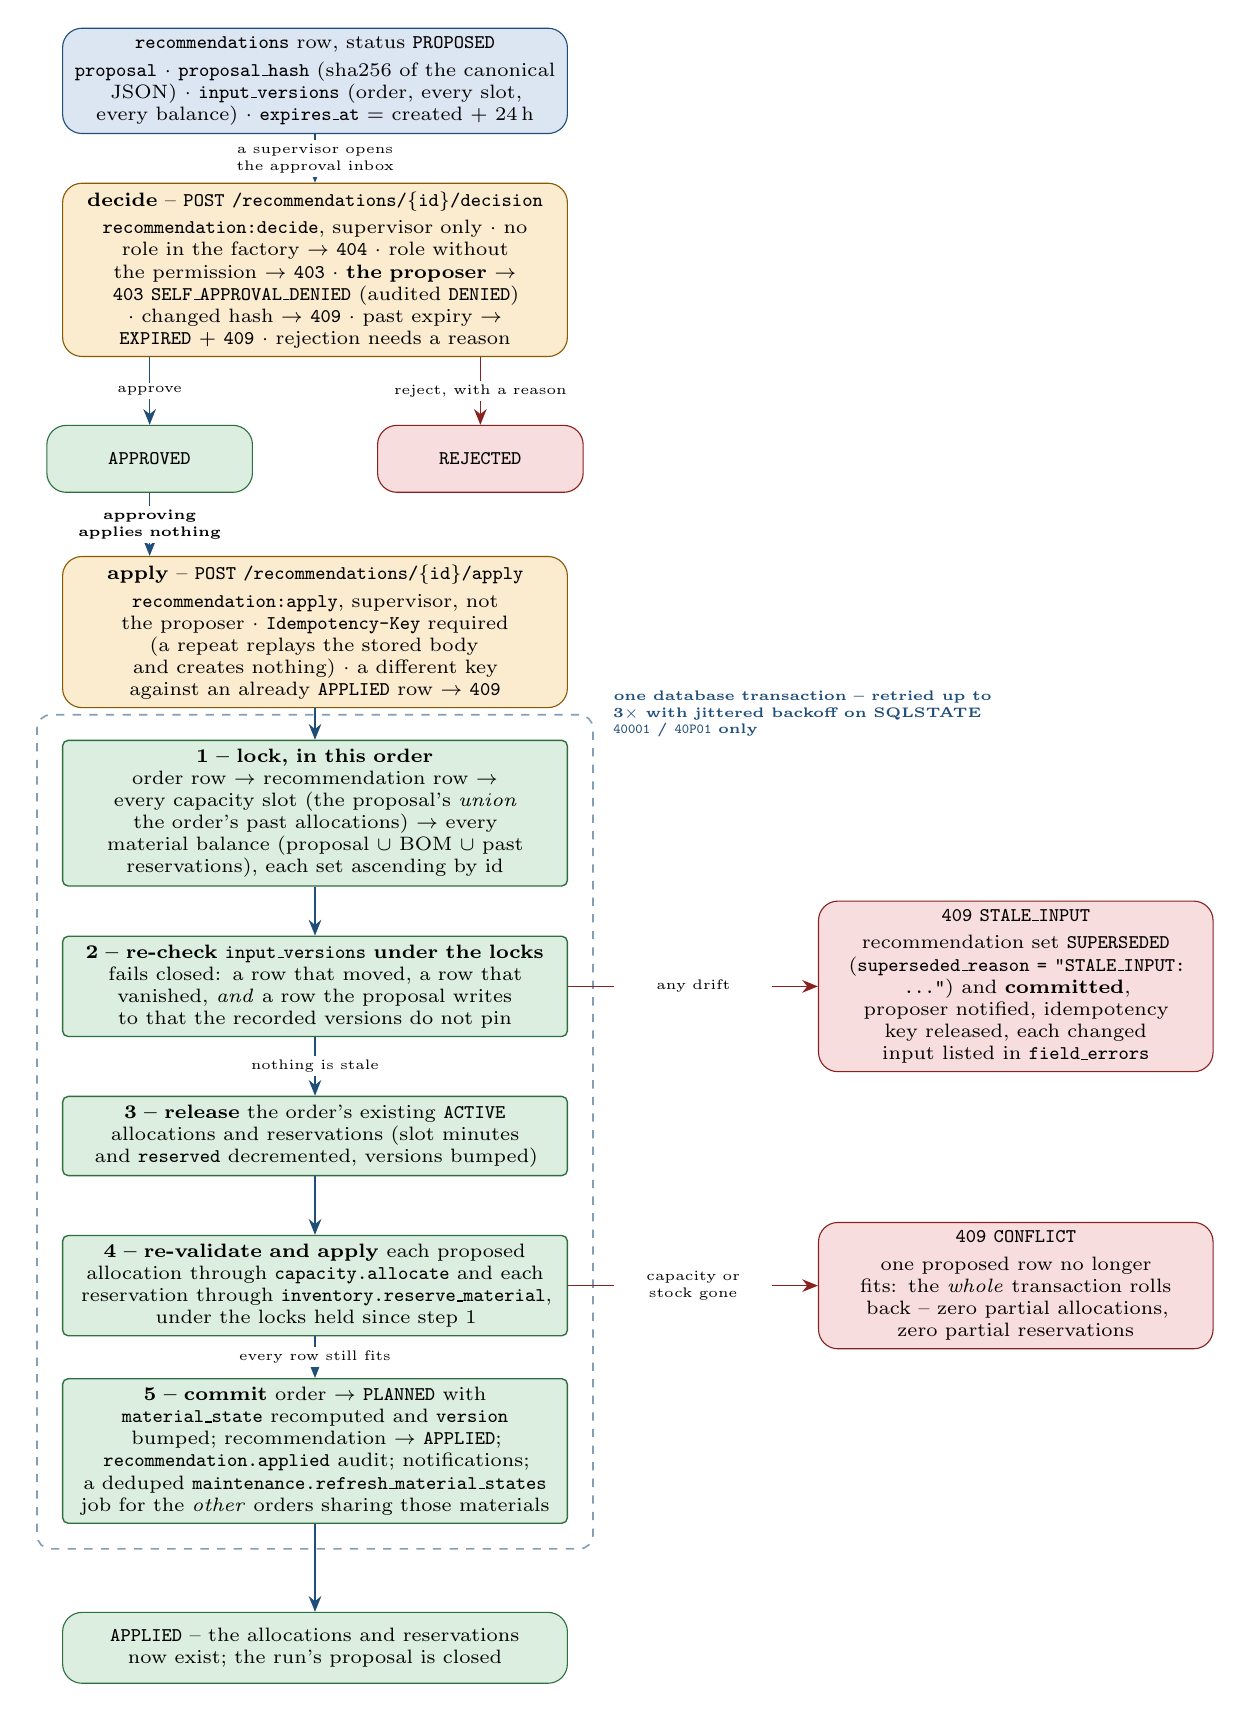
\begin{tikzpicture}[font=\scriptsize]

  \node[state, text width=6.2cm, minimum height=1.25cm] (prop) at (-2.5, 7.2)
    {\texttt{recommendations} row, status \texttt{PROPOSED}\\[2pt]
     \normalfont\scriptsize \texttt{proposal} $\cdot$ \texttt{proposal\_hash} (sha256 of the
     canonical JSON) $\cdot$ \texttt{input\_versions} (order, every slot, every balance) $\cdot$
     \texttt{expires\_at} = created + 24\,h};

  \node[state, draw=lsamber, fill=lsamberd, text width=6.2cm, minimum height=1.6cm]
    (gd) at (-2.5, 4.8)
    {\textbf{decide} -- \texttt{POST /recommendations/\{id\}/decision}\\[2pt]
     \normalfont\scriptsize \texttt{recommendation:decide}, supervisor only $\cdot$
     no role in the factory $\rightarrow$ \texttt{404} $\cdot$ role without the permission
     $\rightarrow$ \texttt{403} $\cdot$ \textbf{the proposer} $\rightarrow$ \texttt{403
     SELF\_APPROVAL\_DENIED} (audited \texttt{DENIED}) $\cdot$ changed hash
     $\rightarrow$ \texttt{409} $\cdot$ past expiry $\rightarrow$ \texttt{EXPIRED} + \texttt{409}
     $\cdot$ rejection needs a reason};

  \node[terminal, text width=2.4cm] (appr) at (-4.6, 2.4) {\texttt{APPROVED}};
  \node[badstate, text width=2.4cm] (rej)  at (-0.4, 2.4) {\texttt{REJECTED}};

  \node[state, draw=lsamber, fill=lsamberd, text width=6.2cm, minimum height=1.4cm]
    (ga) at (-2.5, 0.2)
    {\textbf{apply} -- \texttt{POST /recommendations/\{id\}/apply}\\[2pt]
     \normalfont\scriptsize \texttt{recommendation:apply}, supervisor, not the proposer $\cdot$
     \texttt{Idempotency-Key} required (a repeat replays the stored body and creates
     nothing) $\cdot$ a different key against an already \texttt{APPLIED} row
     $\rightarrow$ \texttt{409}};

  \node[component, text width=6.2cm, minimum height=1.35cm] (s1) at (-2.5,-2.1)
    {\textbf{1 -- lock, in this order}\\ order row $\rightarrow$ recommendation row
     $\rightarrow$ every capacity slot (the proposal's \emph{union} the order's past
     allocations) $\rightarrow$ every material balance (proposal $\cup$ BOM $\cup$ past
     reservations), each set ascending by id};
  \node[component, text width=6.2cm, minimum height=1.15cm] (s2) at (-2.5,-4.3)
    {\textbf{2 -- re-check \texttt{input\_versions} under the locks}\\
     fails closed: a row that moved, a row that vanished, \emph{and} a row the
     proposal writes to that the recorded versions do not pin};
  \node[component, text width=6.2cm, minimum height=1.0cm] (s3) at (-2.5,-6.2)
    {\textbf{3 -- release} the order's existing \texttt{ACTIVE} allocations and
     reservations (slot minutes and \texttt{reserved} decremented, versions bumped)};
  \node[component, text width=6.2cm, minimum height=1.15cm] (s4) at (-2.5,-8.1)
    {\textbf{4 -- re-validate and apply} each proposed allocation through
     \texttt{capacity.allocate} and each reservation through
     \texttt{inventory.reserve\_material}, under the locks held since step~1};
  \node[component, text width=6.2cm, minimum height=1.25cm] (s5) at (-2.5,-10.2)
    {\textbf{5 -- commit} order $\rightarrow$ \texttt{PLANNED} with
     \texttt{material\_state} recomputed and \texttt{version} bumped;
     recommendation $\rightarrow$ \texttt{APPLIED}; \texttt{recommendation.applied}
     audit; notifications; a deduped \texttt{maintenance.refresh\_material\_states}
     job for the \emph{other} orders sharing those materials};

  \begin{scope}[on background layer]
    \node[boundary, fit=(s1)(s2)(s3)(s4)(s5)] (txn) {};
  \end{scope}
  \node[boundlbl, anchor=west, text width=4.8cm]
    at ([shift={(5pt,0pt)}]txn.north east)
    {one database transaction -- retried up to 3$\times$ with jittered backoff on
     SQLSTATE \texttt{40001} / \texttt{40P01} only};

  \node[terminal, text width=6.2cm, minimum height=0.9cm] (done) at (-2.5,-12.7)
    {\texttt{APPLIED} -- the allocations and reservations now exist; the run's
     proposal is closed};

  % ---- failure exits (horizontal, at the y of the raising step) ---------
  \node[badstate, text width=4.8cm, minimum height=1.5cm] (stale) at (6.4,-4.3)
    {\texttt{409 STALE\_INPUT}\\[2pt]
     \normalfont\scriptsize recommendation set \texttt{SUPERSEDED}
     (\texttt{superseded\_reason = "STALE\_INPUT: ..."}) and \textbf{committed},
     proposer notified, idempotency key released, each changed input listed in
     \texttt{field\_errors}};
  \node[badstate, text width=4.8cm, minimum height=1.3cm] (conf) at (6.4,-8.1)
    {\texttt{409 CONFLICT}\\[2pt]
     \normalfont\scriptsize one proposed row no longer fits: the \emph{whole}
     transaction rolls back -- zero partial allocations, zero partial reservations};

  % ---- connectors -------------------------------------------------------
  \draw[trans] (prop.south) -- node[lbl, midway, text width=3.2cm]
      {a supervisor opens the approval inbox} (gd.north);
  \draw[trans] (appr.north |- gd.south) -- node[lbl, midway] {approve} (appr.north);
  \draw[badtrans] (rej.north |- gd.south) -- node[lbl, midway, text width=2.4cm]
      {reject, with a reason} (rej.north);
  \draw[trans] (appr.south) -- node[lbl, midway, text width=3.0cm]
      {\textbf{approving applies nothing}} (appr.south |- ga.north);
  \draw[trans] (ga.south) -- (s1.north);
  \draw[trans] (s1.south) -- (s2.north);
  \draw[trans] (s2.south) -- node[lbl, midway] {nothing is stale} (s3.north);
  \draw[trans] (s3.south) -- (s4.north);
  \draw[trans] (s4.south) -- node[lbl, midway] {every row still fits} (s5.north);
  \draw[trans] (s5.south) -- (done.north);

  \draw[badtrans] (s2.east) -- node[lbl, midway, text width=1.9cm]
      {any drift} (stale.west);
  \draw[badtrans] (s4.east) -- node[lbl, midway, text width=1.9cm]
      {capacity or stock gone} (conf.west);

\end{tikzpicture}
}
\caption{Approval and transactional application. Approving and applying are two
separate acts by a supervisor who is not the proposer, and the application fails
closed on any input drift.}
\label{fig:apply}
\end{figure}

Three properties of figure~\ref{fig:apply} are worth calling out because they
are the ones that are easy to get wrong:

\begin{enumerate}
\item \textbf{The lock set is the union, taken up front.} The transaction locks
  every capacity slot in the proposal \emph{plus} every slot the order has ever
  been allocated to, and every material balance in the proposal \emph{plus} the
  order's BOM materials \emph{plus} every material it has ever reserved --- each
  set ascending by id, before it touches anything. A proposed material without a
  balance row gets one before the lock sweep, so \texttt{reserve\_material} can
  never create and lock a row out of order. Two concurrent applications
  therefore cannot take the same two rows in opposite orders.
\item \textbf{Staleness fails closed.} A row that moved is stale; a row that
  vanished is stale; and a row the proposal would \emph{write to} that
  \texttt{input\_versions} does not pin is stale too --- a missing entry, a key
  that is not a UUID, and a version that is not an integer all count, because
  none of them proves the row has not moved.
\item \textbf{The stale path commits its own status change before failing.} The
  recommendation is set \texttt{SUPERSEDED} with
  \texttt{superseded\_reason = "STALE\_INPUT: \dots"}, audited, the proposer is
  notified, that change is \emph{committed}, the idempotency claim is released
  so the key is not burned on a rejection, and only then does the request fail
  with \texttt{409} listing every changed input in \texttt{field\_errors}.
\end{enumerate}

A mid-apply capacity or stock failure rolls the \emph{whole} transaction back:
zero partial allocations, zero partial reservations. The route owns its session
and retries the whole transaction up to three times with jittered backoff on
SQLSTATE \texttt{40001} and \texttt{40P01} only; everything else propagates.

\subsection{Quality hold, release and shipment eligibility}

A recorded inspection is evaluated against the \emph{active, versioned} policy
and returns a deterministic \texttt{PASS} / \texttt{FAIL} /
\texttt{INSUFFICIENT\_SAMPLE}. A \texttt{FAIL} automatically places an
\texttt{ACTIVE} hold carrying the failing reasons. With \emph{no} approved
policy the inspection is refused (\texttt{409}, ``No approved quality policy'')
--- the system abstains rather than guessing.

Release validates that the inspection is \texttt{FINAL}, \texttt{PASS}, the
latest \texttt{FINAL}, and evaluated against the \emph{current} policy version
(a version mismatch is \texttt{409 STALE\_INPUT}); and it refuses when the
releaser is the inspector (\texttt{403 SELF\_APPROVAL\_DENIED}). Releasing also
releases every active hold. Only then does shipment eligibility change --- and
it changes because the derived predicate now holds, not because anybody said so.

\subsection{Import}

CSV import is upload $\rightarrow$ server validation $\rightarrow$ preview
(first 20 rows plus per-row errors) $\rightarrow$ explicit commit, with the
commit re-running the exact same checks. Either the whole batch commits or
nothing does: a commit-time failure returns \texttt{409} and writes no orders
and no batch status change. Row numbers are physical file lines; the upload
reads at most \texttt{MAX\_FILE\_BYTES + 1} bytes rather than buffering an
unbounded body; a \texttt{csv.Error} becomes a \texttt{REJECTED} batch rather
than a \texttt{500}; and a cell beginning with a spreadsheet formula character
is checked on the \emph{raw} cell and neutralised rather than stored raw.

% =====================================================================
\section{Security}
\label{sec:security}
% =====================================================================

\subsection{Authentication, sessions and tenancy}

OIDC authorization-code flow with PKCE, \texttt{state} and \texttt{nonce}. The
callback passes explicit \texttt{claims\_options} to Authlib requiring the
issuer to equal the discovery issuer, the audience to contain the client id, and
\texttt{sub} to be present --- a fix that closed a real hole found in review, in
which a token with a foreign \texttt{aud} was accepted because its \texttt{azp}
named our client.

Identity is exchanged for an \textbf{opaque, sha256-hashed application session}
with an 8-hour absolute lifetime, rotated after login and after any privilege
change, and revoked on logout. A CSRF middleware checks Origin/Referer
\emph{and} an \texttt{X-CSRF-Token} header on every state-changing
cookie-authenticated request.

Authorization is resolved by shared policy functions
(\texttt{app/auth/scope.py::load\_scoped}) on \emph{every} access path ---
routes, worker tools, retrieval, citations, file downloads and audit views ---
with one consistent rule: \textbf{a resource in a factory the caller holds no
role in is \texttt{404}; an accessible resource missing the required permission
is \texttt{403}.}

\subsection{Threat model}

\texttt{docs/security/threat-model.md} maps each of the specification's threats
to a STRIDE category, an implemented control and the test that exercises it.
Summarised:

\begin{table}[h]
\centering\small
\caption{Threats, controls, and the tests that prove them.}
\begin{tabularx}{\linewidth}{@{}L{3.0cm}YL{4.3cm}@{}}
\toprule
\textbf{Threat} & \textbf{Control} & \textbf{Proven by}\\
\midrule
Cross-factory / order access &
\texttt{load\_scoped} on every path; 404 vs 403 split &
\texttt{test\_idor\_matrix.py} (generated from the live app's routes), \texttt{test\_order\_access.py}, \texttt{test\_document\_access.py}\\
Prompt injection in SOPs &
read/compute-only tools, untrusted tool-result handling, candidate-action and
evidence-id whitelists, bounded calls &
\texttt{test\_prompt\_injection.py} (real RM loop vs the real adversarial document), \texttt{test\_document\_tool.py}\\
Forged / stale approval &
self-approval denial, hash and version binding re-checked inside the locking
transaction &
\texttt{test\_approvals.py}, \texttt{test\_approval\_rules.py}\\
Duplicate consumption &
sorted-id row locks, required idempotency keys, unique \texttt{(task\_id)} on results &
\texttt{test\_apply\_concurrency.py}, \texttt{test\_reservation\_concurrency.py}, \texttt{test\_worker\_kill.py}\\
SQL injection / XSS &
parameterized SQLAlchemy only, no model SQL, React text nodes, CSP &
\texttt{xss.test.tsx}, \texttt{test\_headers\_and\_limits.py}\\
Malicious uploads &
size cap, type sniffing, quarantine-until-processed, no public originals &
\texttt{test\_document\_pipeline.py}\\
SSRF / exfiltration &
no tool accepts a URL; outbound calls only to settings-derived addresses &
tool sets are closed and defined per agent in code\\
Secret disclosure &
\texttt{SecretStr}/environment only, structlog key dropping, provider-payload redaction, repository scanning &
\texttt{test\_redaction.py} (34 cases), \texttt{scripts/secret-scan.sh}\\
Cost / request abuse &
per-user and per-IP token buckets, per-run model and token budgets, max active runs per factory &
\texttt{test\_headers\_and\_limits.py}, \texttt{test\_budget.py}\\
Worker / service impersonation &
constant-time bearer service token, never a cookie; route absent from the public API &
\texttt{test\_internal\_dispatch.py}\\
\bottomrule
\end{tabularx}
\end{table}

\subsection{Prompt injection: what the adversarial test actually proves}

\texttt{data/synthetic/adversarial/injection-sop.md} is a document that asks the
model to approve without review, to call \texttt{delete\_all\_records}, to reveal
a secret, and to cite a fabricated chunk id. It is loaded through the
\emph{real} document pipeline and retrieved by the \emph{real} RM agent loop,
driven by a deliberately obedient scripted model. The observed outcome:

\begin{itemize}
\item the injected text reaches the model only inside a \texttt{tool\_result},
  as data;
\item the \texttt{delete\_all\_records} call returns an unknown-tool error and
  has no effect;
\item the fabricated chunk id fails validation, one repair turn is offered, it
  fails again, and the run \textbf{degrades} with
  \texttt{error\_code=INVALID\_AGENT\_OUTPUT} --- with \texttt{evidence\_refs}
  reduced back to the untouched deterministic set and
  \texttt{recommended\_actions} byte-identical to the agent's own deterministic
  assessment.
\end{itemize}

That is the honest claim: \textbf{injection cannot escalate}, because the model
was never the authority. It is not a claim that injection can be detected.
Detection alone is not a security boundary, and this project does not treat it
as one.

\subsection{Scans (recorded runs)}

\begin{quote}\small\ttfamily
\$ bash scripts/secret-scan.sh\\
{[secret-scan]} OK: no high-risk secret patterns found in 413 tracked files\\[4pt]
\$ uvx pip-audit --requirement /tmp/requirements.txt\\
Resolved 114 packages in 2ms\\
No known vulnerabilities found\\[4pt]
\$ npm audit --omit=dev --audit-level=high\\
found 0 vulnerabilities
\end{quote}

One documented, reviewed exclusion: the scan excludes paths under a
\texttt{tests/} directory, because this repository's own tests deliberately
contain literal fake \texttt{sk-ant-\dots}-shaped strings in order to test
\emph{this project's} redaction and error-handling code. Each such string is
listed by file and line in \texttt{docs/security/scan-results.md}.

\subsection{Accepted residual risks}

\begin{itemize}
\item \textbf{No row-level security yet.} Tenant isolation is enforced in the
  application layer and covered by a route-generated IDOR matrix. Database RLS
  --- policies keyed on a transaction-local \texttt{organization\_id}, a
  non-owner non-\texttt{BYPASSRLS} runtime role, and pool-reuse tests --- is a
  documented \textbf{required gate before any multi-organization pilot}, not
  something quietly dropped.
\item \textbf{Rate limits are per process.} Behind more than one API instance
  each enforces its own budget; a shared store would be needed to cap the true
  aggregate.
\item \textbf{Structural upload scan, no antivirus engine} and \textbf{no OCR}.
\item \textbf{The development IdP is not a real IdP} --- shared password,
  in-memory state, a signing key regenerated on every restart, no TLS. It
  refuses to start outside development/test.
\item \textbf{Append-only audit permissions are not cryptographic
  tamper-proofing.} Stronger immutable archival is a later production
  requirement.
\end{itemize}

% =====================================================================
\section{Responsible AI implementation}
% =====================================================================

The full treatment is \texttt{docs/assessment/responsible-ai.md}, with the model
and data cards alongside it. The implemented positions:

\textbf{Worker privacy.} Operator identifiers are pseudonymous alias codes
(\texttt{KTN-OP-017}) created by the seed generator; no name, contact detail,
health information, protected attribute or disciplinary record exists anywhere
in the schema. Observations reach the IE agent \emph{aggregated per operation};
operator aliases are not in the run snapshot, no tool returns one, and a test
asserts no summary, finding or action contains one. A defect belongs to an
operation and an inspection, never to a person.

\textbf{No individual ranking, ever.} The IE agent's only action is
\texttt{IE\_REVIEW} --- ``review method and staffing at \texttt{<operation>} on
\texttt{<line>}'' --- targeting a process constraint and a staffing
\emph{level}. There is no code path that ranks, scores or compares individuals.

\textbf{Explainability through evidence, not through model introspection.}
Every finding carries evidence references that resolve to a record with its
version or a document with its version, page and section, and every citation is
re-authorized when opened. The product does not display model reasoning as an
explanation, and it does not display a model-produced confidence number as if it
were a calibrated probability.

\textbf{Transparency about what produced a value.} The provider label is carried
from the adapter to the API to the screen. In this build every agent summary
shows \emph{``Test fixture --- not a live AI model''}, because that is the
truth.

\textbf{Abstention.} No approved policy $\rightarrow$ nothing can be
dispositioned and the order cannot ship. No inspection $\rightarrow$ quality is
\emph{unknown}, not \emph{pass}. Unknown consumption $\rightarrow$
\texttt{coverage\_days} is \texttt{None} with an explanation, not zero. A
missing dependency $\rightarrow$ a degraded result naming what is missing, not a
fabricated success.

\textbf{Human oversight and correction.} Consequential changes require approval
by someone other than the proposer; rejection requires a reason; the original
proposal and its history are retained; and every decision, application, release
and policy change is audited with before/after summaries.

\textbf{Fairness --- and the limits of what was tested.} The harness runs the
\emph{same} order through the four-agent flow twice, changing only its customer,
and compares the stored \texttt{proposal\_hash}. Two \emph{different} orders are
not a valid comparison, because the hash covers a payload embedding the order
id. In the smoke run, 2 of 2 pairs were byte-identical. That shows the
deterministic flow does not let customer identity change the allocation under a
deterministic provider. It is \textbf{not} an audit of fairness across any
protected characteristic; it cannot show whether a live model would let a
customer's identity leak into its phrasing or tool choices; and a 100\% pass
rate here is necessary, not sufficient.

\textbf{Limitations statement.} Synthetic tests and aggregate checks do not
prove fairness for a real workforce. Before real factory data is accepted, the
project commits to a provider-data review, a retention schedule, a documented
deletion process and an incident procedure --- all drafted in
\texttt{docs/assessment/responsible-ai.md} --- and treats legal obligations as a
separate jurisdiction-specific review, never as a compliance claim.

% =====================================================================
\section{Evaluation results}
\label{sec:eval}
% =====================================================================

\statusbox{What these numbers are, exactly}{%
The table below is the \textbf{smoke run} of the evaluation harness:
\texttt{--embedder hashing --scenarios 2}, against an isolated test database,
recorded in \texttt{docs/IMPLEMENTATION\_STATUS.md}. It was run to verify the
harness end to end, not to produce the project's headline numbers. The real run
--- \texttt{make eval}, i.e.\ \texttt{--embedder fastembed --scenarios 12}
against \texttt{linesense\_eval} --- is \textbf{PENDING (needs user approval or
CI)} and has never been executed here.
\texttt{docs/evaluation/results/} is deliberately empty rather than holding a
hashing-embedder run presented as canonical.}

\begin{table}[h]
\centering\small
\caption{Evaluation smoke run (\texttt{--embedder hashing --scenarios 2}).}
\begin{tabularx}{\linewidth}{@{}L{5.4cm}ccY@{}}
\toprule
\textbf{Target} & \textbf{Threshold} & \textbf{Actual} & \textbf{Met}\\
\midrule
\texttt{retrieval\_hybrid\_recall\_at\_5} & 0.85 & 0.711 &
\textbf{no} --- expected: the hashing embedder has no semantics, and 2 of the 45
test questions are legitimately out-of-scope BYG documents\\
\texttt{entities\_micro\_f1} & 0.90 & 0.991 & yes\\
\texttt{classification\_tfidf\_macro\_f1} & 0.80 & 0.835 & yes\\
\texttt{calculations\_all\_pass} & 1 & 1 & yes\\
\bottomrule
\end{tabularx}
\end{table}

Other sections of the same smoke run:

\begin{itemize}
\item \textbf{Agents (2 scenarios).} All three approaches --- deterministic
  baseline, single-agent baseline, four-agent flow --- scored material-conflict
  accuracy 1.0. The four-agent flow's \texttt{capacity\_sufficient}
  approximation scored 0.5 (1 of 2). Both figures are noise at $n=2$; the second
  is additionally an acknowledged approximation, because
  \texttt{unscheduled\_units} can be driven by a capacity \emph{or} a material
  shortfall and the two are not separately exposed.
  \emph{The single-agent baseline can never detect a material conflict
  (\texttt{material\_conflict\_pred} is always false) because it never sees the
  RM agent's assessment --- that is the comparison's whole point, and the report
  says so in its own \texttt{single\_agent\_baseline\_note} field.}
\item \textbf{Security.} 2 of 2 prompt-injection cases blocked; 3 of 3 abstention
  checks passed.
\item \textbf{Fairness.} 2 of 2 customer-swap pairs byte-identical.
\end{itemize}

Three real bugs were found and fixed while getting the harness green, which is
itself evidence that the harness exercises the real code path: agent scenarios
were creating runs with no snapshot (the orchestrator correctly refused every
one); the in-memory single-agent baseline crashed on the run-budget reservation;
and the fairness section was comparing two different orders' hashes, which can
never match.

\subsection{Functional verification that \emph{was} executed}

Test execution in this project was focused rather than exhaustive, under a
machine heat and workload policy that forbids running full suites locally. What
follows are runs actually recorded in \texttt{docs/IMPLEMENTATION\_STATUS.md},
with their exact pass counts:

\begin{table}[h]
\centering\small
\caption{A selection of recorded focused test runs (see the status file for the
full log, including the command line and the database used for each).}
\begin{tabularx}{\linewidth}{@{}YL{2.2cm}@{}}
\toprule
\textbf{Scope} & \textbf{Result}\\
\midrule
Schema, grants and tenancy constraints (\texttt{test\_schema.py}) & 11 passed\\
Domain calculations and the reference fixtures, plus Hypothesis property tests & 78 passed\\
Job queue, worker runtime, leases and fencing & 30 passed (of a 98-pass integration run)\\
Agent protocol, internal dispatch, analysis API, executor & 52 passed\\
RM and planning agents; orchestrator; two-agent flow & 31 + 11 + 1 passed\\
IE and quality agents, four-agent graph, order report & 108 passed\\
Approvals, apply concurrency, approval rules & 6 + 9, then 35 after fix round 1\\
Document pipeline, hybrid search, document access, agent document tool & 17 + 20 + 2 passed\\
Entities, classifier, summaries, notes API, status summary & 48 passed\\
Headers/rate limits, IDOR matrix, prompt injection, worker-kill resilience & 81 passed\\
Query-count regressions (five list endpoints) + approvals & 19 passed\\
Dashboard and administration APIs & 13 passed\\
Whole web suite (\texttt{npx vitest run}) & 34 files, 123 passed\\
\bottomrule
\end{tabularx}
\end{table}

Two of those runs are worth singling out because they test the property rather
than the implementation:

\begin{itemize}
\item \texttt{test\_two\_applications\_contend\_for\_the\_last\_slot\_minutes}
  creates a \emph{real} overlap using \texttt{pg\_sleep} while the lock is held,
  repeated five times, and asserts exactly one application succeeds and capacity
  is never exceeded.
\item \texttt{tests/resilience/test\_worker\_kill.py} \texttt{SIGKILL}s a real
  worker subprocess mid-task, waits for the lease to expire, lets another worker
  reclaim it, and asserts exactly one result exists and the run still finalizes.
\end{itemize}

A mutation check was also recorded for the locking code: removing
\texttt{FOR UPDATE} from \texttt{lock\_balances} makes all 11 concurrency tests
fail --- so those tests are testing the lock, not passing by accident.

\subsection{Backup and restore (a real, recorded exercise)}

\begin{quote}\small\ttfamily
\$ time bash scripts/backup.sh linesense\_dev\\
\dots\\
bash scripts/backup.sh linesense\_dev  0.43s user 0.19s system 70\% cpu 0.877 total\\[4pt]
\$ time bash scripts/restore.sh .local/backups/20260920T080449Z.tar.enc\\
{[restore]} verifying row counts against the backup manifest\\
{[restore]} verifying document\_versions.storage\_key files exist\\
{[restore]} verifying material\_balances against the movement ledger\\
{[restore]} verification passed.\\
bash scripts/restore.sh "\$latest"  0.48s user 0.22s system 46\% cpu 1.507 total
\end{quote}

Backup \textbf{0.877\,s} for a 368{,}672-byte encrypted archive; restore plus
full three-part verification \textbf{1.507\,s}. This is evidence the mechanism
works at demonstration scale --- it is \emph{not} a claim about restore time at
real factory data volumes.

\textbf{An honest gap in that exercise:} the database it ran against had not had
\texttt{make seed --with-documents} run, so \texttt{document\_versions} was 0 and
verification step 2 (every \texttt{ACTIVE}/\texttt{SUPERSEDED}
\texttt{storage\_key} exists in the restored store) had zero rows to check ---
its code path was not exercised by this run, and no automated test currently
exercises it either.

% =====================================================================
\section{Reliability, performance and deployment}
% =====================================================================

\subsection{Reliability}

Background work runs through a PostgreSQL job table with
\texttt{FOR UPDATE SKIP LOCKED} claiming, short leases with heartbeats, and
fenced completion (figure~\ref{fig:jobstate}). \textbf{Delivery is at least once
and is documented as such}; exactly-once is never advertised. A worker that dies
mid-task is recovered either by its lease expiring or by \texttt{reconcile\_once},
which re-enqueues \texttt{orchestrator.advance} for any run quiet for more than
30 seconds with no runnable job of its own.

Error text stored in \texttt{last\_error} is the exception class plus the first
500 characters of its message, capped at 2{,}000, never a traceback or local
variables; for SQLAlchemy statement errors only the driver exception's class and
first message line are stored, never the SQL; and engines are created with
\texttt{hide\_parameters=True} so bound values stay out of error messages.

\subsection{Efficiency}

RM, IE and quality run concurrently; planning waits for RM and IE. Dashboard
cards are computed in deterministic SQL --- exactly six statements per request,
enforced by a query-count-bound integration test --- and \textbf{no LLM call is
made when a dashboard is opened}. Query-count regression tests cover five list
endpoints and caught a real N+1 in
\texttt{app.domain.approvals.service.list\_recommendations}; another caught and
fixed an N+1 in the order history route. Embeddings are stored with their model
name, so chunks embedded by a different model are never compared.

\subsection{Performance: not measured}

\statusbox{Performance targets are targets, and none of them has been measured}{%
The specification's initial targets --- non-AI API p95 under 500\,ms at 20
concurrent users, analysis acknowledgement p95 under 1\,s, a four-agent run
usually under 60\,s within a 120\,s deadline --- are \textbf{targets to evaluate
against, not results}. The load generator (\texttt{scripts/perf\_smoke.py}), its
\texttt{make perf} target and its documentation are complete and were
smoke-checked (\texttt{--help}, \texttt{ruff}, \texttt{mypy} all clean), but
\textbf{no load has ever been generated}: this project's machine heat and
workload policy explicitly forbids it on this laptop. There are therefore no
latency numbers in this report, and no plausible-looking placeholder has been
substituted for them. The exact commands to produce them are in
\texttt{docs/evaluation/performance.md}.}

\subsection{Deployment}

\begin{landscape}
\begin{figure}[p]
\centering
\resizebox{\linewidth}{!}{% Deployment view: the single-host Docker Compose topology.
% NOTE: statically validated only (`make infra-check`); never built or run in
% the environment that produced this report.
%
% Host services sit on a fixed grid (rows y = 5.0 | 1.4 | -2.2); external
% systems sit outside the dashed host boundary on the far left (browser,
% backups) and far right (LLM provider).  Corridors y = -0.4 and y = -4.6 and
% x = 4.6 carry the connectors that would otherwise cross a node.
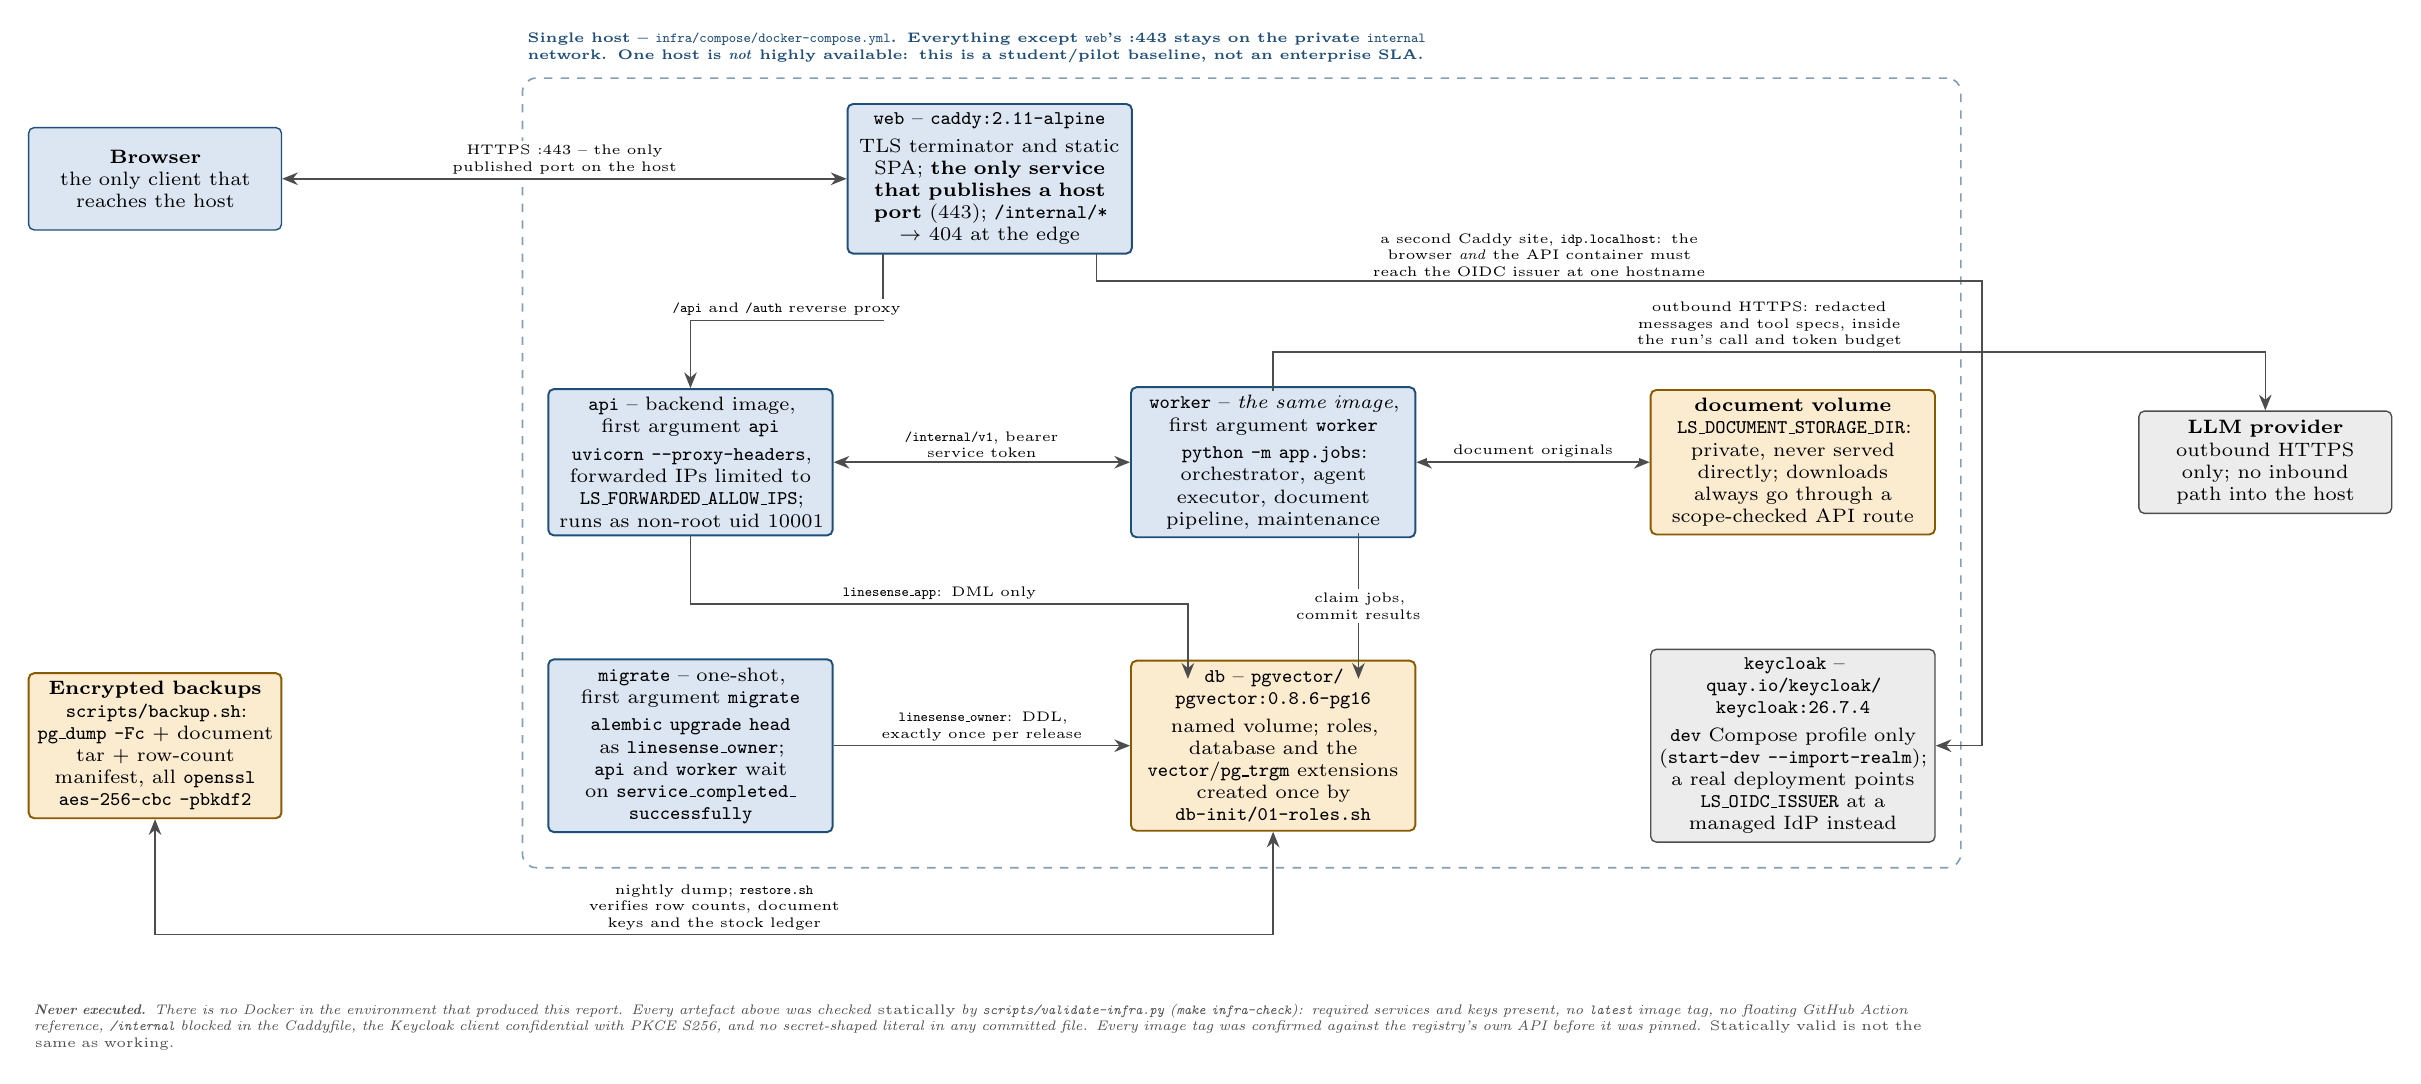
\begin{tikzpicture}[font=\scriptsize]

  % ---------- host services ----------------------------------------------
  \node[container, text width=3.4cm, minimum height=1.9cm] (web) at (-1.0, 5.0)
    {\textbf{\texttt{web}} -- \texttt{caddy:2.11-alpine}\\[2pt]
     \normalfont\scriptsize TLS terminator and static SPA; \textbf{the only service
     that publishes a host port} (443); \texttt{/internal/*} $\rightarrow$ 404 at the
     edge};

  \node[container, text width=3.4cm, minimum height=1.8cm] (api) at (-4.8, 1.4)
    {\textbf{\texttt{api}} -- backend image, first argument \texttt{api}\\[2pt]
     \normalfont\scriptsize \texttt{uvicorn --proxy-headers}, forwarded IPs limited
     to \texttt{LS\_FORWARDED\_ALLOW\_IPS}; runs as non-root uid 10001};

  \node[container, text width=3.4cm, minimum height=1.8cm] (worker) at (2.6, 1.4)
    {\textbf{\texttt{worker}} -- \emph{the same image}, first argument
     \texttt{worker}\\[2pt]
     \normalfont\scriptsize \texttt{python -m app.jobs}: orchestrator, agent
     executor, document pipeline, maintenance};

  \node[container, text width=3.4cm, minimum height=1.7cm] (mig) at (-4.8,-2.2)
    {\textbf{\texttt{migrate}} -- one-shot, first argument \texttt{migrate}\\[2pt]
     \normalfont\scriptsize \texttt{alembic upgrade head} as
     \texttt{linesense\_owner}; \texttt{api} and \texttt{worker} wait on
     \texttt{service\_completed\_}\\\texttt{successfully}};

  \node[store, text width=3.4cm, minimum height=1.7cm] (db) at (2.6,-2.2)
    {\textbf{\texttt{db}} -- \texttt{pgvector/}\\\texttt{pgvector:0.8.6-pg16}\\[2pt]
     \normalfont\scriptsize named volume; roles, database and the
     \texttt{vector}/\texttt{pg\_trgm} extensions created once by
     \texttt{db-init/01-roles.sh}};

  \node[external, text width=3.4cm, minimum height=1.7cm] (kc) at (9.2,-2.2)
    {\textbf{\texttt{keycloak}} -- \texttt{quay.io/keycloak/}\\\texttt{keycloak:26.7.4}\\[2pt]
     \normalfont\scriptsize \texttt{dev} Compose profile only
     (\texttt{start-dev --import-realm}); a real deployment points
     \texttt{LS\_OIDC\_ISSUER} at a managed IdP instead};

  \node[store, text width=3.4cm, minimum height=1.5cm] (vol) at (9.2, 1.4)
    {\textbf{document volume}\\ \normalfont\scriptsize
     \texttt{LS\_DOCUMENT\_STORAGE\_DIR}: private, never served directly; downloads
     always go through a scope-checked API route};

  \begin{scope}[on background layer]
    \node[boundary, fit=(web)(api)(worker)(mig)(db)(kc)(vol)] (host) {};
  \end{scope}
  \node[boundlbl, anchor=south west, text width=12.0cm]
    at ([shift={(0pt,3pt)}]host.north west)
    {Single host -- \texttt{infra/compose/docker-compose.yml}. Everything except
     \texttt{web}'s :443 stays on the private \texttt{internal} network. One host
     is \emph{not} highly available: this is a student/pilot baseline, not an
     enterprise SLA.};

  % ---------- external systems --------------------------------------------
  \node[person, text width=3.0cm, minimum height=1.3cm] (browser) at (-11.6, 5.0)
    {\textbf{Browser}\\ \normalfont\scriptsize the only client that reaches the host};
  \node[store, text width=3.0cm, minimum height=1.6cm] (bak) at (-11.6,-2.2)
    {\textbf{Encrypted backups}\\ \normalfont\scriptsize \texttt{scripts/backup.sh}:
     \texttt{pg\_dump -Fc} + document tar + row-count manifest, all
     \texttt{openssl aes-256-cbc -pbkdf2}};
  \node[external, text width=3.0cm, minimum height=1.3cm] (llm) at (15.2, 1.4)
    {\textbf{LLM provider}\\ \normalfont\scriptsize outbound HTTPS only; no inbound
     path into the host};

  % ---------- connectors ---------------------------------------------------
  \draw[biflow] (browser.east) -- node[lbl, above, midway, text width=3.4cm]
      {HTTPS :443 -- the only published port on the host} (web.west);

  % web -> api, along the corridor y = 3.2
  \draw[flow] (-2.354, 4.05) -- (-2.354, 3.2) --
      node[lbl, above, midway, text width=3.0cm]
      {\texttt{/api} and \texttt{/auth} reverse proxy} (-4.8,3.2) -- (api.north);

  % web -> keycloak, along the corridor y = 3.7
  \draw[flow] (0.354, 4.05) -- (0.354, 3.7) --
      node[lbl, above, midway, text width=5.0cm]
      {a second Caddy site, \texttt{idp.localhost}: the browser \emph{and} the API
       container must reach the OIDC issuer at one hostname} (11.6,3.7)
      -- (11.6,-2.2) -- (kc.east);

  \draw[biflow] (api.east) -- node[lbl, above, midway, text width=2.8cm]
      {\texttt{/internal/v1}, bearer service token} (worker.west);

  % api -> db, along the corridor y = -0.4
  \draw[flow] (api.south) -- (-4.8,-0.4) --
      node[lbl, above, midway, text width=2.8cm]
      {\texttt{linesense\_app}: DML only} (1.517,-0.4) -- (1.517,-1.35);

  % worker -> db, pure vertical
  \draw[flow] (3.683, 0.5) -- node[lbl, midway, text width=2.4cm]
      {claim jobs, commit results} (3.683,-1.35);

  % worker -> document volume
  \draw[biflow] (worker.east) -- node[lbl, above, midway, text width=2.6cm]
      {document originals} (vol.west);

  % worker -> LLM provider, along the corridor y = 2.8 (leaves the host)
  \draw[flow] (2.6, 2.3) -- (2.6, 2.8) --
      node[lbl, above, midway, text width=4.2cm]
      {outbound HTTPS: redacted messages and tool specs, inside the run's
       call and token budget} (15.2,2.8) -- (llm.north);

  \draw[flow] (mig.east) -- node[lbl, above, midway, text width=2.8cm]
      {\texttt{linesense\_owner}: DDL, exactly once per release} (db.west);

  \draw[biflow] (db.south) -- (2.6,-4.6) --
      node[lbl, above, midway, text width=3.2cm]
      {nightly dump; \texttt{restore.sh} verifies row counts, document keys and the
       stock ledger} (-11.6,-4.6) -- (bak.south);

  \node[note, anchor=north west, text width=24.0cm] at (-13.2,-5.4)
    {\textbf{Never executed.} There is no Docker in the environment that produced
     this report. Every artefact above was checked \emph{statically} by
     \texttt{scripts/validate-infra.py} (\texttt{make infra-check}): required
     services and keys present, no \texttt{latest} image tag, no floating GitHub
     Action reference, \texttt{/internal} blocked in the Caddyfile, the Keycloak
     client confidential with PKCE~S256, and no secret-shaped literal in any
     committed file. Every image tag was confirmed against the registry's own API
     before it was pinned. \emph{Statically valid is not the same as working.}};

\end{tikzpicture}
}
\caption{The single-host Compose deployment. Statically validated, never run.}
\label{fig:deploy}
\end{figure}
\end{landscape}

The deployment sequence is: build and scan immutable images $\rightarrow$ back
up $\rightarrow$ run migrations \emph{exactly once as a release job}, never
competitively in every server worker $\rightarrow$ deploy API, worker and assets
$\rightarrow$ readiness checks (\texttt{/api/health/live},
\texttt{/api/health/ready}, worker heartbeat) $\rightarrow$ authenticated smoke
flow $\rightarrow$ observe. Compose models this with a one-shot \texttt{migrate}
service that \texttt{api} and \texttt{worker} wait on via
\texttt{service\_completed\_successfully}.

Rollback is deliberately \emph{not} ``run the down migration''. A destructive
down migration is not a safe default rollback plan; the documented approach is
backward-compatible expand/contract migrations, with application rollback
requiring database compatibility.

One design consequence is recorded honestly as a demo-only limitation: the OIDC
issuer must be reachable at the \emph{same} hostname from the browser and from
the API container, which is solved here with a second Caddy site
(\texttt{idp.localhost}) and a Compose network alias. A real deployment does not
have this problem, because a real hostname gets a publicly trusted certificate.

\textbf{A single host is not highly available.} The demonstration objectives ---
daily encrypted backups, recovery point up to 24 hours, restore within 4 hours
--- are planning objectives, not an SLA, and a commercial SLA would need a
stronger design and a contractual review.

% =====================================================================
\section{Commercialization}
\label{sec:commercial}
% =====================================================================

The full plan is \texttt{docs/assessment/commercialization.md}. In summary:

\textbf{Target and positioning.} Apparel factories that currently reconcile
spreadsheet, ERP, stores, IE and quality information by hand. LineSense is
positioned as a \emph{decision-support layer with traceable recommendations},
not as an ERP replacement and not as an autonomous scheduler. Buyer interest
must be validated with production managers, factory owners and operations/quality
leads. \textbf{No market validation is claimed from this architecture.}

\textbf{Pricing (hypotheses, not validated rates).}

\begin{table}[h]
\centering\small
\caption{Illustrative tiers in USD. These are hypotheses from the project
specification, not current vendor prices or validated market rates.}
\begin{tabular}{@{}lll@{}}
\toprule
\textbf{Tier} & \textbf{Proposed price} & \textbf{Proposed scope}\\
\midrule
Pilot & \$99 / factory / month & up to 5 lines, 10 users, 500 analysis\\
 & & runs per month, CSV imports\\
\addlinespace
Growth & \$249 / factory / month & up to 20 lines, 30 users, 2{,}000 runs\\
 & & per month, richer reporting\\
\addlinespace
Enterprise & quoted & multiple factories, connector work,\\
 & & isolated deployment, negotiated support\\
\bottomrule
\end{tabular}
\end{table}

Every tier is described against \emph{implemented} features, with anything else
marked explicitly as roadmap. Onboarding and connector work is charged
separately after estimating effort. A run's maximum model and tool budget,
document storage allowance, retention and overage behaviour are defined before a
tier is offered. \textbf{Unlimited AI use is never promised.}

\textbf{Cost model.} Monthly service delivery cost is allocated compute +
database + storage and backups + monitoring + model and embedding usage +
support labour + identity/email costs, and gross margin is
$(\text{revenue} - \text{service delivery cost}) / \text{revenue}$.

\statusbox{Per-run model cost cannot be quoted from this build}{%
Token counts recorded by this repository come from the \texttt{fixture}
provider, which computes them as \texttt{len(json.dumps(\dots)) // 4} --- a
cheap deterministic stand-in, \textbf{not a tokenizer and not provider usage}.
They are usable as a \emph{method} --- measure \texttt{tokens\_used} per run,
multiply by the provider's published per-token prices, add the embedding cost
--- and they are not usable as a cost figure. Any quoted per-run cost must come
from a live-provider run with current published prices verified at the time of
quoting.}

\textbf{Deployment options.} Single-tenant SaaS hosted by the vendor, or
customer-hosted Compose on the customer's own VM for factories that will not let
operational data leave the site.

\textbf{Pilot plan.} Measure time to identify a blocker, time spent preparing an
order-status report, stale/missing-data rate, proposal acceptance rate and
supervisor-rated usefulness --- before and after. Progress from synthetic demo
$\rightarrow$ read-only pilot $\rightarrow$ supervised actions $\rightarrow$
integrations, and only after validation at each step. \textbf{No productivity
percentage is promised before before/after evidence exists.}

% =====================================================================
\section{Limitations, and what has not been verified}
\label{sec:not-verified}
% =====================================================================

\subsection{Never executed in this environment}

\begin{table}[h]
\centering\small
\caption{Everything that is not verified, with the exact missing dependency.}
\begin{tabularx}{\linewidth}{@{}L{4.8cm}YL{3.4cm}@{}}
\toprule
\textbf{Not verified} & \textbf{Why} & \textbf{Missing dependency}\\
\midrule
Live LLM provider run & no API key exists in this environment; the Anthropic
adapter is exercised only against in-test stub SDK clients &
\texttt{LS\_ANTHROPIC\_API\_KEY}\\
Full evaluation (\texttt{make eval}) & the real \texttt{fastembed} run needs a
$\sim$100\,MB model download plus a full embedding and query pass &
user approval or CI\\
Load test (\texttt{make perf}) & sustained concurrent load for 60\,s is exactly
what the machine heat policy forbids locally & user approval or CI\\
Full test suites (\texttt{make test}, \texttt{test-integration},
\texttt{test-all}, \texttt{security}) & same policy; only the files covering each
change were run & user approval or CI\\
Any Docker operation & no Docker in this environment; images were never built or
started & a Docker host or CI\\
Keycloak realm import and the hosted TLS login flow & depends on the above &
a Docker host\\
Browser end-to-end flows and screenshots & \textbf{Task 24 was dropped by the
user} as a scope decision & a reinstated E2E task\\
Real-factory validation of the formulas & synthetic data only; an IE/domain owner
must validate production assumptions & a domain owner\\
Official report template & never supplied (\S\ref{sec:template-gap}) & the
lecturer's template\\
Lecturer-approved domain list & never supplied; the manufacturing domain is
assumed, not confirmed & the approved list\\
\bottomrule
\end{tabularx}
\end{table}

\subsection{Known functional limitations}

\begin{itemize}
\item \textbf{No row-level security}; application-layer tenancy only (a
  documented pre-pilot gate).
\item \textbf{No OCR}; scanned or image-only PDFs are rejected with a message
  rather than partially parsed. \textbf{No antivirus engine}; a structural
  marker scan only.
\item \textbf{No approximate vector index.} Vector search is an exact scan ---
  adequate at 30 documents, not at scale.
\item \textbf{Single-instance rate limits}, in-process token buckets.
\item \textbf{In-app notifications only}; no email or SMS.
\item \textbf{No live ERP/MES connector.} The adapter interface
  (\texttt{fetch\_changes}, \texttt{normalize}, \texttt{validate},
  \texttt{apply\_idempotently}, \texttt{checkpoint}) is documented and nothing is
  connected.
\item \textbf{One style per order} (ADR-0007); no \texttt{order\_items}.
\item A note's \texttt{unresolved} entity list and its classifier version at
  creation time are not persisted --- there are no columns for them --- so the
  list is only ever populated on the create response and the version shown is
  always the current process's.
\item The IE screen can only mark outliers on observations recorded in the
  current session, because no endpoint lists historical observations.
\item \texttt{CANCELLED} exists in the \texttt{jobs} schema and is set by no code
  path.
\end{itemize}

\subsection{Future work, in the order it should be done}

\begin{enumerate}
\item Run the full verification set in CI and publish the artefacts: the full
  suites, \texttt{make eval} with \texttt{fastembed}, \texttt{make perf}, and the
  Docker build and Compose smoke flow.
\item Configure a provider key and record a live multi-agent run, then repeat
  the agent and fairness evaluation three times to report variance rather than a
  single number.
\item Implement database row-level security before onboarding a second
  organization.
\item Reinstate browser end-to-end coverage of the critical flows and capture the
  screenshots this submission lacks.
\item Add an approximate vector index and a shared rate-limit store before any
  multi-instance deployment.
\item Have an IE/domain owner validate the production assumptions behind the
  formulas before any real-factory use.
\end{enumerate}

% =====================================================================
\section{Conclusion}
% =====================================================================

LineSense AI implements what the assignment asked for and, where it could not
verify something, says so. Four agents really do interact --- the planning agent
revises its allocation because the RM agent's number contradicted it, driven by
a deterministic comparison rather than a model's opinion. The protocol between
them is versioned, schema-checked and server-verified against the run it claims
to belong to. Retrieval is genuinely hybrid and genuinely access-controlled
before content reaches a model. Approval integrity is enforced by row locks and
version pinning rather than by convention, and is proved by tests that create
real contention.

The part of the work that is easiest to undervalue is the part that refuses to
claim things: the source label on every value, the abstention paths that return
\emph{unknown} instead of a plausible number, the degraded result that names
what was lost, the evaluation directory that is empty rather than populated with
a smoke run dressed up as a result, and the list in \S\ref{sec:not-verified}. A
decision-support system for a factory is only worth deploying if the people using
it can tell which of its statements are facts. That property was designed in
from the first task, and it is the one this report most wants to be judged on.

% =====================================================================
\section*{References}
\addcontentsline{toc}{section}{References}
% =====================================================================

Only sources actually used while building this system are listed.

\begin{enumerate}[leftmargin=2em]
\item pgvector --- open-source vector similarity search for PostgreSQL.
  \url{https://github.com/pgvector/pgvector}
\item PostgreSQL 17 documentation, \texttt{SELECT} (\texttt{FOR UPDATE SKIP
  LOCKED}). \url{https://www.postgresql.org/docs/current/sql-select.html}
\item PostgreSQL 17 documentation, row security policies.
  \url{https://www.postgresql.org/docs/17/ddl-rowsecurity.html}
\item OWASP Cheat Sheet Series --- LLM Prompt Injection Prevention.
  \url{https://cheatsheetseries.owasp.org/cheatsheets/LLM_Prompt_Injection_Prevention_Cheat_Sheet.html}
\item OWASP Cheat Sheet Series --- Session Management.
  \url{https://cheatsheetseries.owasp.org/cheatsheets/Session_Management_Cheat_Sheet.html}
\item FastAPI --- deployment concepts.
  \url{https://fastapi.tiangolo.com/deployment/concepts/}
\item Vite --- getting started guide. \url{https://vite.dev/guide/}
\item Playwright documentation (referenced by the plan for browser end-to-end
  testing; that task was dropped). \url{https://playwright.dev/docs/intro}
\item Keycloak --- running Keycloak in a container.
  \url{https://www.keycloak.org/server/containers}
\end{enumerate}

\appendix
\clearpage
% =====================================================================
\section{Role permission matrix}
\label{app:roles}
% =====================================================================

Generated from \texttt{app.auth.policy.PERMISSIONS} by
\texttt{scripts/gen\_role\_matrix.py}; regenerate rather than hand-editing.
Columns: IE = \texttt{ie\_engineer}, OA = \texttt{org\_admin}, PL =
\texttt{planner}, QM = \texttt{quality\_manager}, SK = \texttt{storekeeper}, SV =
\texttt{supervisor}, VW = \texttt{viewer}.

\begin{table}[h]
\centering\small
\begin{tabular}{@{}lccccccc@{}}
\toprule
\textbf{Permission} & IE & OA & PL & QM & SK & SV & VW\\
\midrule
\texttt{admin:manage}           &   & x &   &   &   &   &  \\
\texttt{analysis:read}          & x & x & x & x & x & x & x\\
\texttt{analysis:run}           &   &   & x &   &   & x &  \\
\texttt{audit:read}             &   & x &   &   &   & x &  \\
\texttt{capacity:read}          & x & x & x & x & x & x & x\\
\texttt{document:read}          & x & x & x & x & x & x & x\\
\texttt{document:upload}        & x & x &   & x &   & x &  \\
\texttt{ie:read}                & x & x & x & x & x & x & x\\
\texttt{ie:write}               & x &   &   &   &   &   &  \\
\texttt{inventory:read}         & x & x & x & x & x & x & x\\
\texttt{inventory:write}        &   &   &   &   & x &   &  \\
\texttt{note:create}            & x &   & x & x & x & x &  \\
\texttt{order:cancel}           &   &   &   &   &   & x &  \\
\texttt{order:create}           &   &   & x &   &   & x &  \\
\texttt{order:dispatch}         &   &   &   &   &   & x &  \\
\texttt{order:import}           &   &   & x &   &   & x &  \\
\texttt{order:read}             & x & x & x & x & x & x & x\\
\texttt{order:transition}       &   &   & x &   &   & x &  \\
\texttt{quality:hold}           &   &   &   & x &   &   &  \\
\texttt{quality:inspect}        &   &   &   & x &   &   &  \\
\texttt{quality:read}           & x & x & x & x & x & x & x\\
\texttt{quality:release}        &   &   &   & x &   &   &  \\
\texttt{recommendation:apply}   &   &   &   &   &   & x &  \\
\texttt{recommendation:decide}  &   &   &   &   &   & x &  \\
\bottomrule
\end{tabular}
\end{table}

\clearpage
% =====================================================================
\section{API surface}
% =====================================================================

66 public paths / 70 operations, exported deterministically to
\texttt{contracts/openapi.json} (OpenAPI 3.1.0, 151 component schemas) and used
to generate the TypeScript client. Grouped:

\begin{table}[h]
\centering\small
\begin{tabularx}{\linewidth}{@{}L{3.0cm}Y@{}}
\toprule
\textbf{Group} & \textbf{Representative endpoints}\\
\midrule
Identity & \texttt{GET /auth/login}, \texttt{GET /auth/callback}, \texttt{POST /auth/logout}, \texttt{GET /api/v1/me}\\
Health & \texttt{GET /api/health/live}, \texttt{GET /api/health/ready}\\
Orders & \texttt{GET|POST /api/v1/factories/\{f\}/orders}, \texttt{GET /api/v1/orders/\{id\}}, transition and progress commands, \texttt{GET /api/v1/orders/\{id\}/history}\\
Imports & create batch, validate/preview, commit, row errors, template download\\
Analysis & \texttt{POST /api/v1/orders/\{id\}/analyses}, \texttt{GET /api/v1/runs/\{id\}}, \texttt{GET /api/v1/runs/\{id\}/events}, \texttt{GET /api/v1/orders/\{id\}/runs}, cancel, retry\\
Planning / capacity & \texttt{GET /api/v1/factories/\{f\}/lines}, \texttt{GET /api/v1/factories/\{f\}/capacity}\\
Inventory & material overview, ledger, receipts, lot acceptance, issues, corrections, reservations, release\\
IE & \texttt{POST} observations, mark outlier, operator aliases, \texttt{GET .../ie/\{line\}/\{style\}/analysis}\\
Quality & inspections, holds, releases, defect trends, shipment facts\\
Recommendations & scoped list, detail, \texttt{POST .../decision}, \texttt{POST .../apply}\\
Documents / search & upload, list, detail, version detail, download, \texttt{GET /factories/\{f\}/search}, \texttt{GET /citations/\{chunk\_id\}}\\
NLP & \texttt{POST|GET /api/v1/factories/\{f\}/notes}, \texttt{GET /api/v1/orders/\{id\}/status-summary}\\
Dashboard / admin / audit / notifications & factory dashboard, memberships, role grant/revoke, deactivate, policies, settings, scoped audit list, notifications list and mark-read\\
Internal (not in the public document) & \texttt{POST /internal/v1/agent-tasks}, \texttt{GET /internal/v1/agent-tasks/\{id\}}\\
\bottomrule
\end{tabularx}
\end{table}

Error bodies are uniform: \texttt{code}, a safe \texttt{message}, optional
\texttt{field\_errors}, \texttt{trace\_id} and an optional server-controlled
retry hint. \texttt{401}/\texttt{403} are used correctly, \texttt{404} avoids
disclosing inaccessible resources, \texttt{409} covers stale and conflicting
writes, \texttt{422} covers invalid input and \texttt{429} covers rate limits.

\clearpage
% =====================================================================
\section{Command reference}
% =====================================================================

\begin{table}[h]
\centering\small
\begin{tabularx}{\linewidth}{@{}L{3.6cm}Y@{}}
\toprule
\textbf{Target} & \textbf{What it does}\\
\midrule
\texttt{make bootstrap} & initialise the project-local PostgreSQL cluster, copy \texttt{.env}, \texttt{uv sync}\\
\texttt{make db-start} / \texttt{db-stop} / \texttt{db-init} / \texttt{db-reset-test} & manage \emph{only} the project-local cluster on port 55432\\
\texttt{make migrate} & \texttt{alembic upgrade head}\\
\texttt{make migration-check} & upgrade $\rightarrow$ downgrade $\rightarrow$ upgrade $\rightarrow$ \texttt{alembic check} against the test database\\
\texttt{make seed} & deterministic synthetic dataset + the 30-document SOP corpus\\
\texttt{make idp} & the development-only OIDC provider (port 8090)\\
\texttt{make worker} & the durable worker (\texttt{python -m app.jobs})\\
\texttt{make lint} / \texttt{typecheck} / \texttt{format} & ruff + eslint / mypy + tsc / auto-format\\
\texttt{make test} / \texttt{test-integration} / \texttt{test-all} & unit and web / real-PostgreSQL integration / both\\
\texttt{make contracts} / \texttt{contracts-check} & export OpenAPI + protocol schemas + TS client / detect drift\\
\texttt{make datasets-check} & validate the synthetic corpus and labelled datasets\\
\texttt{make docs-check} & every relative documentation link resolves\\
\texttt{make infra-check} & static validation of Compose, Caddyfile, realm and CI workflow\\
\texttt{make security} & secret scan + dependency audit + the \texttt{security}-marked suite\\
\texttt{make eval} & the full evaluation with the real embedder\\
\texttt{make perf} & the load generator (never run here)\\
\texttt{make backup} / \texttt{restore-check} & encrypted backup / timed backup-restore-verify exercise\\
\texttt{make build} & backend import check + production web build\\
\texttt{make web-install} / \texttt{web-dev} / \texttt{web-test} / \texttt{web-build} & frontend equivalents\\
\bottomrule
\end{tabularx}
\end{table}

There is no \texttt{make dev} target (each process is started explicitly --- see
\texttt{docs/user-guide.md} \S4) and no \texttt{make test-e2e} target (browser
end-to-end testing was dropped).

\clearpage
% =====================================================================
\section{Architecture decision records}
% =====================================================================

\begin{table}[h]
\centering\small
\begin{tabularx}{\linewidth}{@{}L{1.3cm}Y@{}}
\toprule
\textbf{ADR} & \textbf{Decision}\\
\midrule
0001 & Modular monolith plus a separate worker; agents are components, not microservices\\
0002 & PostgreSQL + pgvector as the single store; exact vector search first\\
0003 & PostgreSQL job table with \texttt{FOR UPDATE SKIP LOCKED}, leases, fencing and at-least-once delivery\\
0004 & OIDC + PKCE + opaque server sessions + CSRF double-check; a development-only OIDC provider locally, a Keycloak realm for Compose\\
0005 & A custom versioned HTTP/JSON agent protocol --- explicitly not A2A, not MCP\\
0006 & One \texttt{LLMClient} boundary: Anthropic \texttt{claude-opus-5} with server-side refusal fallbacks, a deterministic \texttt{fixture} provider for CI, and a \texttt{disabled} degraded mode\\
0007 & One style per order; a ledger plus a lockable \texttt{material\_balances} row; embeddings on \texttt{chunks}; one \texttt{approvals} row per recommendation\\
0008 & A local environment without Docker or Java: a project-local PostgreSQL cluster on port 55432, and Compose/Keycloak validated statically only\\
\bottomrule
\end{tabularx}
\end{table}

\vfill
\notebox{Where to look next}{%
\texttt{docs/user-guide.md} --- setup and every screen and workflow.\quad
\texttt{docs/IMPLEMENTATION\_STATUS.md} --- the dated log of what was built and
what was actually run.\quad
\texttt{docs/assessment/completion-matrix.md} --- every requirement and
acceptance gate with a verdict and evidence.\quad
\texttt{docs/assessment/} --- commercialization, responsible AI, model and data
cards, video script, contribution and AI-assistance logs, licences.}

\end{document}
